\documentclass[conference]{IEEEtran}
\IEEEoverridecommandlockouts

\usepackage{cite}
\usepackage{amsmath,amssymb,amsfonts}
\usepackage{algorithmic}
\usepackage{graphicx}
\usepackage{textcomp}
\usepackage{xcolor}
\usepackage{booktabs}
\usepackage{hyperref}
\usepackage{siunitx}
\usepackage{multirow}
\graphicspath{{../../}{./}{results/figures/}{figures/}}

% Paper numbers — auto-generated from empirical score arrays, do not edit by hand
\IfFileExists{paper_numbers_p2.tex}{% Auto-generated by src/final_phase2.py — DO NOT EDIT BY HAND
% Author: Kushal Sarkar (Phase 2 Lead Integration)
% All values computed directly from verified results/scores/*.npy files
\newcommand{\BaseRateTest}{0.1317\%}
\newcommand{\BaseRateVal}{0.1001\%}
\newcommand{\NTest}{56{,}962}
\newcommand{\NVal}{56{,}961}
\newcommand{\NFraudTest}{75}
\newcommand{\NFraudVal}{57}
\newcommand{\PRAUCTestPCA}{0.7425}
\newcommand{\PRAUCValPCA}{0.7066}
\newcommand{\ROCAUCTestPCA}{0.9303}
\newcommand{\RecallFPRTightPCA}{0.7600}
\newcommand{\RecallFPRHalfPctPCA}{0.7733}
\newcommand{\RecallFPROnePctPCA}{0.7733}
\newcommand{\PrecCapHalfPctPCA}{0.2000}
\newcommand{\PrecKHundredPCA}{0.5700}
\newcommand{\PRAUCTestLOF}{0.4478}
\newcommand{\PRAUCValLOF}{0.4069}
\newcommand{\ROCAUCTestLOF}{0.9048}
\newcommand{\RecallFPRTightLOF}{0.6533}
\newcommand{\RecallFPRHalfPctLOF}{0.7200}
\newcommand{\RecallFPROnePctLOF}{0.7467}
\newcommand{\PrecCapHalfPctLOF}{0.1860}
\newcommand{\PrecKHundredLOF}{0.4700}
\newcommand{\PRAUCTestGMM}{0.2679}
\newcommand{\PRAUCValGMM}{0.1038}
\newcommand{\ROCAUCTestGMM}{0.9391}
\newcommand{\RecallFPRTightGMM}{0.3333}
\newcommand{\RecallFPRHalfPctGMM}{0.6667}
\newcommand{\RecallFPROnePctGMM}{0.7333}
\newcommand{\PrecCapHalfPctGMM}{0.1719}
\newcommand{\PrecKHundredGMM}{0.3100}
\newcommand{\PRAUCTestOCSVM}{0.1322}
\newcommand{\PRAUCValOCSVM}{0.0613}
\newcommand{\ROCAUCTestOCSVM}{0.9604}
\newcommand{\RecallFPRTightOCSVM}{0.0000}
\newcommand{\RecallFPRHalfPctOCSVM}{0.6933}
\newcommand{\RecallFPROnePctOCSVM}{0.8133}
\newcommand{\PrecCapHalfPctOCSVM}{0.1649}
\newcommand{\PrecKHundredOCSVM}{0.1600}
\newcommand{\PRAUCTestIFOREST}{0.0577}
\newcommand{\PRAUCValIFOREST}{0.0330}
\newcommand{\ROCAUCTestIFOREST}{0.9567}
\newcommand{\RecallFPRTightIFOREST}{0.0133}
\newcommand{\RecallFPRHalfPctIFOREST}{0.3467}
\newcommand{\RecallFPROnePctIFOREST}{0.5867}
\newcommand{\PrecCapHalfPctIFOREST}{0.0772}
\newcommand{\PrecKHundredIFOREST}{0.0700}
\newcommand{\PRAUCTestAE}{0.3574}
\newcommand{\PRAUCValAE}{0.2272}
\newcommand{\ROCAUCTestAE}{0.9021}
\newcommand{\RecallFPRTightAE}{0.5333}
\newcommand{\RecallFPRHalfPctAE}{0.6800}
\newcommand{\RecallFPROnePctAE}{0.8000}
\newcommand{\PrecCapHalfPctAE}{0.1754}
\newcommand{\PrecKHundredAE}{0.4000}
\newcommand{\PRAUCTestDAE}{0.4818}
\newcommand{\PRAUCValDAE}{0.2935}
\newcommand{\ROCAUCTestDAE}{0.9322}
\newcommand{\RecallFPRTightDAE}{0.7067}
\newcommand{\RecallFPRHalfPctDAE}{0.7733}
\newcommand{\RecallFPROnePctDAE}{0.7733}
\newcommand{\PrecCapHalfPctDAE}{0.2035}
\newcommand{\PrecKHundredDAE}{0.5300}
\newcommand{\PRAUCTestHOne}{0.1724}
\newcommand{\PRAUCValHOne}{0.1159}
\newcommand{\ROCAUCTestHOne}{0.9398}
\newcommand{\RecallFPRTightHOne}{0.2400}
\newcommand{\RecallFPRHalfPctHOne}{0.7467}
\newcommand{\RecallFPROnePctHOne}{0.7867}
\newcommand{\PrecCapHalfPctHOne}{0.1930}
\newcommand{\PrecKHundredHOne}{0.3000}
\newcommand{\PRAUCTestHTwo}{0.4818}
\newcommand{\PRAUCValHTwo}{0.2935}
\newcommand{\ROCAUCTestHTwo}{0.9322}
\newcommand{\RecallFPRTightHTwo}{0.7067}
\newcommand{\RecallFPRHalfPctHTwo}{0.7733}
\newcommand{\RecallFPROnePctHTwo}{0.7733}
\newcommand{\PrecCapHalfPctHTwo}{0.2035}
\newcommand{\PrecKHundredHTwo}{0.5300}
\newcommand{\PRAUCTestHThree}{0.4541}
\newcommand{\PRAUCValHThree}{0.3913}
\newcommand{\ROCAUCTestHThree}{0.9127}
\newcommand{\RecallFPRTightHThree}{0.6800}
\newcommand{\RecallFPRHalfPctHThree}{0.8000}
\newcommand{\RecallFPROnePctHThree}{0.8000}
\newcommand{\PrecCapHalfPctHThree}{0.2070}
\newcommand{\PrecKHundredHThree}{0.4800}
}{% Auto-generated by src/final_phase2.py — DO NOT EDIT BY HAND
% Author: Kushal Sarkar (Phase 2 Lead Integration)
% All values computed directly from verified results/scores/*.npy files
\newcommand{\BaseRateTest}{0.1317\%}
\newcommand{\BaseRateVal}{0.1001\%}
\newcommand{\NTest}{56{,}962}
\newcommand{\NVal}{56{,}961}
\newcommand{\NFraudTest}{75}
\newcommand{\NFraudVal}{57}
\newcommand{\PRAUCTestPCA}{0.7425}
\newcommand{\PRAUCValPCA}{0.7066}
\newcommand{\ROCAUCTestPCA}{0.9303}
\newcommand{\RecallFPRTightPCA}{0.7600}
\newcommand{\RecallFPRHalfPctPCA}{0.7733}
\newcommand{\RecallFPROnePctPCA}{0.7733}
\newcommand{\PrecCapHalfPctPCA}{0.2000}
\newcommand{\PrecKHundredPCA}{0.5700}
\newcommand{\PRAUCTestLOF}{0.4478}
\newcommand{\PRAUCValLOF}{0.4069}
\newcommand{\ROCAUCTestLOF}{0.9048}
\newcommand{\RecallFPRTightLOF}{0.6533}
\newcommand{\RecallFPRHalfPctLOF}{0.7200}
\newcommand{\RecallFPROnePctLOF}{0.7467}
\newcommand{\PrecCapHalfPctLOF}{0.1860}
\newcommand{\PrecKHundredLOF}{0.4700}
\newcommand{\PRAUCTestGMM}{0.2679}
\newcommand{\PRAUCValGMM}{0.1038}
\newcommand{\ROCAUCTestGMM}{0.9391}
\newcommand{\RecallFPRTightGMM}{0.3333}
\newcommand{\RecallFPRHalfPctGMM}{0.6667}
\newcommand{\RecallFPROnePctGMM}{0.7333}
\newcommand{\PrecCapHalfPctGMM}{0.1719}
\newcommand{\PrecKHundredGMM}{0.3100}
\newcommand{\PRAUCTestOCSVM}{0.1322}
\newcommand{\PRAUCValOCSVM}{0.0613}
\newcommand{\ROCAUCTestOCSVM}{0.9604}
\newcommand{\RecallFPRTightOCSVM}{0.0000}
\newcommand{\RecallFPRHalfPctOCSVM}{0.6933}
\newcommand{\RecallFPROnePctOCSVM}{0.8133}
\newcommand{\PrecCapHalfPctOCSVM}{0.1649}
\newcommand{\PrecKHundredOCSVM}{0.1600}
\newcommand{\PRAUCTestIFOREST}{0.0577}
\newcommand{\PRAUCValIFOREST}{0.0330}
\newcommand{\ROCAUCTestIFOREST}{0.9567}
\newcommand{\RecallFPRTightIFOREST}{0.0133}
\newcommand{\RecallFPRHalfPctIFOREST}{0.3467}
\newcommand{\RecallFPROnePctIFOREST}{0.5867}
\newcommand{\PrecCapHalfPctIFOREST}{0.0772}
\newcommand{\PrecKHundredIFOREST}{0.0700}
\newcommand{\PRAUCTestAE}{0.3574}
\newcommand{\PRAUCValAE}{0.2272}
\newcommand{\ROCAUCTestAE}{0.9021}
\newcommand{\RecallFPRTightAE}{0.5333}
\newcommand{\RecallFPRHalfPctAE}{0.6800}
\newcommand{\RecallFPROnePctAE}{0.8000}
\newcommand{\PrecCapHalfPctAE}{0.1754}
\newcommand{\PrecKHundredAE}{0.4000}
\newcommand{\PRAUCTestDAE}{0.4818}
\newcommand{\PRAUCValDAE}{0.2935}
\newcommand{\ROCAUCTestDAE}{0.9322}
\newcommand{\RecallFPRTightDAE}{0.7067}
\newcommand{\RecallFPRHalfPctDAE}{0.7733}
\newcommand{\RecallFPROnePctDAE}{0.7733}
\newcommand{\PrecCapHalfPctDAE}{0.2035}
\newcommand{\PrecKHundredDAE}{0.5300}
\newcommand{\PRAUCTestHOne}{0.1724}
\newcommand{\PRAUCValHOne}{0.1159}
\newcommand{\ROCAUCTestHOne}{0.9398}
\newcommand{\RecallFPRTightHOne}{0.2400}
\newcommand{\RecallFPRHalfPctHOne}{0.7467}
\newcommand{\RecallFPROnePctHOne}{0.7867}
\newcommand{\PrecCapHalfPctHOne}{0.1930}
\newcommand{\PrecKHundredHOne}{0.3000}
\newcommand{\PRAUCTestHTwo}{0.4818}
\newcommand{\PRAUCValHTwo}{0.2935}
\newcommand{\ROCAUCTestHTwo}{0.9322}
\newcommand{\RecallFPRTightHTwo}{0.7067}
\newcommand{\RecallFPRHalfPctHTwo}{0.7733}
\newcommand{\RecallFPROnePctHTwo}{0.7733}
\newcommand{\PrecCapHalfPctHTwo}{0.2035}
\newcommand{\PrecKHundredHTwo}{0.5300}
\newcommand{\PRAUCTestHThree}{0.4541}
\newcommand{\PRAUCValHThree}{0.3913}
\newcommand{\ROCAUCTestHThree}{0.9127}
\newcommand{\RecallFPRTightHThree}{0.6800}
\newcommand{\RecallFPRHalfPctHThree}{0.8000}
\newcommand{\RecallFPROnePctHThree}{0.8000}
\newcommand{\PrecCapHalfPctHThree}{0.2070}
\newcommand{\PrecKHundredHThree}{0.4800}
}

\def\BibTeX{{\rm B\kern-.05em{\sc i\kern-.025em b}\kern-.08em
    T\kern-.1667em\lower.7ex\hbox{E}\kern-.125emX}}

\begin{document}

\title{Card Fraud Triage via Deep Autoencoders and Hybrid Latent Density Scoring:\\
Phase 2 — Deep Learning \& Hybrid Anomaly Detection\\
{\footnotesize Team T033, Section A, Project 26 — Rishihood University}}

\author{
\IEEEauthorblockN{Kushal Sarkar\textsuperscript{1},
                  Krishna Pramod Dubale\textsuperscript{2},
                  Apoorva Choudhary\textsuperscript{3},
                  Vani Rudra\textsuperscript{4},
                  Prachee Dhar\textsuperscript{5}}
\IEEEauthorblockA{School of Technology, Rishihood University, Sonipat, Haryana, India\\
Enrollment: \textsuperscript{1}2401020033
            \textsuperscript{2}2401010239
            \textsuperscript{3}2401010092
            \textsuperscript{4}2401010490
            \textsuperscript{5}2401010330\\
Faculty Advisors: Shobhit Johri, Arun Chauhan, Ashwin Tewary}
}

\maketitle

\begin{abstract}
In Phase 1 of Project T033, classical anomaly detection established linear Principal Component Analysis (PCA) reconstruction error as the leading baseline (PR-AUC \PRAUCTestPCA{}, Recall@0.5\% FPR \RecallFPRHalfPctPCA{} on the held-out test split), outperforming Gaussian Mixture Models (GMM, PR-AUC \PRAUCTestGMM{}) and Isolation Forests (PR-AUC \PRAUCTestIFOREST{}). In this Phase 2 study, we investigate two fundamental hypotheses: (1) whether non-linear manifold learning via Deep Undercomplete and Denoising Autoencoders (DAE) improves fraud triage over linear PCA, and (2) whether fitting a Gaussian Mixture Model in the compressed latent bottleneck ($\mathbf{z} \in \mathbb{R}^8$) eliminates the curse of dimensionality while retaining explicit probabilistic density scoring.
Evaluating ten models on the chronologically split ULB benchmark (\NTest{} test transactions, \NFraudTest{} test frauds, base rate \BaseRateTest{}), we demonstrate that the Denoising Autoencoder ($\sigma=0.2$, PR-AUC \PRAUCTestDAE{}) significantly outperforms full-space GMM ($\Delta = +0.2139$, $p < 0.05$) and doubles fraud recall at tight false-alarm budgets (\RecallFPRTightDAE{} vs.\ \RecallFPRTightGMM{} at FPR $\le 0.1\%$). However, linear PCA remains the highest performing standalone detector on this PCA-anonymized dataset because deep architectures exhibit partial over-generalization to anomalies. Furthermore, standalone latent-space density estimation (Hybrid H1, PR-AUC \PRAUCTestHOne{}) degrades due to non-volume-preserving encoder compression and latent non-Gaussianity. Crucially, multi-objective DAGMM-lite (Hybrid H3), which augments latent coordinates with reconstruction error and cosine angle distortion, achieves the highest test recall at FPR $\le 0.5\%$ across all evaluated methods (\RecallFPRHalfPctHThree{}, catching 60 of 75 frauds). We provide complete 5-seed stability profiles, stratified bootstrap confidence intervals, ablation breakdowns, and operational review triage policies.
\end{abstract}

\begin{IEEEkeywords}
fraud triage, deep autoencoders, denoising autoencoders, Gaussian mixture models, latent space density, DAGMM-lite, class imbalance, precision-recall
\end{IEEEkeywords}

%%% ─── 1. Introduction ────────────────────────────────────────────────────────
% Section: Phase 2 Introduction
% Author: Krishna Pramod Dubale (Task P2_01)
% IEEE Conference Paper Section - Card Fraud Triage (Phase 2)

\section{Introduction}
\label{sec:p2_introduction}

Financial transaction networks process billions of digital payments daily while operating under persistent threats from evolving adversarial fraud syndicates \cite{dalpozzolo2018credit, leborgne2022handbook}. In retail banking, automated transaction triage confronts three fundamental structural constraints: extreme class imbalance ($<0.2\%$ base rate), multi-week verification lag during dispute resolution, and continuous concept drift driven by circadian consumer spending and shifting fraud patterns \cite{dalpozzolo2015calibrating, lucas2020dataset}. Under these constraints, purely supervised classification is highly vulnerable to temporal look-ahead leakage and severe overfitting on stale fraud signatures.

\subsection{Recap of Phase 1 Findings}
\label{sec:p1_recap}
In Phase~1 of Project T033, we investigated classical unsupervised anomaly detection and parametric density estimation on the benchmark ULB dataset (284,807 transactions across 48 continuous hours). Models were trained exclusively on legitimate records under a strict chronological partition (60\% train, 20\% validation, 20\% test). The empirical results established that linear \emph{Principal Component Analysis (PCA) reconstruction error} achieved the highest triage performance ($\text{PR-AUC} = 0.7425$, $\text{Recall@FPR=0.5\%} = 0.7733$ on the held-out test set), significantly outperforming full-space density estimation via Gaussian Mixture Models ($\text{PR-AUC} = 0.4142$) and classical baselines including Local Outlier Factor (0.4478), One-Class SVM (0.1322), and Isolation Forest (0.0577). Extensive statistical auditing revealed that severe leptokurtosis and heavy tails across PCA components degrade parametric Gaussian assumptions in the ambient 30-dimensional feature space, while subspace projection acts as a robust noise filter.

\subsection{Phase 2 Motivation and Research Objectives}
\label{sec:p2_motivation}
Although PCA reconstruction error dominated Phase~1, PCA is mathematically restricted to planar linear subspaces. Real-world financial transaction distributions occupy non-linear, multi-scale manifolds embedded within the high-dimensional ambient space. Phase~2 extends our investigation by deploying deep neural representation architectures to address the central research question:
\begin{quote}
\emph{Does learning a non-linear compressed representation using a Deep Undercomplete Autoencoder, combined with latent-space Gaussian Mixture density estimation, significantly improve fraud triage compared with classical linear and density baselines?}
\end{quote}

To answer this question, Phase~2 develops:
\begin{enumerate}
    \item \textbf{Undercomplete and Denoising Autoencoders:} Non-linear neural architectures that optimize reconstruction Mean Squared Error (MSE) over legitimate transactions, learning the geometry of normal spending while suppressing noise via stochastic corruption.
    \item \textbf{Decoupled Hybrid Architectures:} Three novel hybrid formulations:
    \begin{itemize}
        \item \textbf{Hybrid 1 ($H_1$, Latent-GMM):} Estimating multimodal probability densities $-\log p(\mathbf{z})$ exclusively within the compressed autoencoder bottleneck space $\mathbf{z} \in \Real{}^k$.
        \item \textbf{Hybrid 2 ($H_2$, Score Fusion):} Convex combination of standardized reconstruction error and ambient density scores.
        \item \textbf{Hybrid 3 ($H_3$, DAGMM-Lite):} Density estimation over joint latent embeddings augmented with non-linear reconstruction distance features.
    \end{itemize}
    \item \textbf{Strict Anti-Leakage DL Pipeline:} PyTorch streaming data pipeline enforcing pure legitimate training tensors, validation-legitimate early stopping hygiene, and feature-variance balancing.
    \item \textbf{Systematic Ablation Study:} Quantifying the independent impact of bottleneck dimensionality, regularization (dropout, weight decay), denoising noise level ($\sigma$), and training sample volume.
\end{enumerate}

\subsection{Paper Organization}
The remainder of this report is organized as follows: Section~\ref{sec:p2_dl_literature} provides the deep learning literature review and formalizes the research gap; Section~\ref{sec:p2_dl_data_pipeline} details the deep learning data pipeline and anti-leakage invariants; Section~\ref{sec:p2_architecture} presents the autoencoder network design and regularization study; Section~\ref{sec:p2_hybrid_theory} analyzes the theoretical foundations of latent-space density modeling ($H_1$); Section~\ref{sec:p2_hybrid} introduces hybrid architectures ($H_2, H_3$) and the master ablation study; Section~\ref{sec:p2_validation} provides rigorous technical validation and paired bootstrap tests; and Section~\ref{sec:master_synthesis} synthesizes overall operational findings and concluding recommendations.


%%% ─── 2. Deep Learning Literature Review ─────────────────────────────────────
% Section: Deep Learning Literature Review
% Author: Krishna Pramod Dubale (Task P2_01)
% IEEE Conference Paper Section - Card Fraud Triage (Phase 2)

\section{Deep Learning Literature Review \& Theoretical Gap}
\label{sec:p2_dl_literature}

\subsection{Autoencoders and Manifold Learning}
Dimensionality reduction using neural networks originates from the foundational work of Hinton and Salakhutdinov \cite{hinton2006reducing}, who demonstrated that deep multilayer autoencoders discover compact non-linear coordinate systems capable of reconstructing complex manifolds with significantly lower error than classical PCA. An autoencoder parameterizes an encoder $f_{\boldsymbol{\theta}}: \Real{}^d \to \Real{}^k$ and decoder $g_{\boldsymbol{\phi}}: \Real{}^k \to \Real{}^d$ with bottleneck dimension $k \ll d$. When all hidden activations are linear and optimized under Mean Squared Error (MSE), the learned latent subspace is identical to the principal subspace discovered by PCA \cite{bourlard1988auto, baldi1989neural}. Introducing non-linear activation functions (ReLU, Tanh) allows the autoencoder to model continuous curved sub-manifolds embedded within the ambient transaction space $\Real{}^d$.

To prevent autoencoders from learning trivial identity mappings, Vincent et al. \cite{vincent2008extracting} introduced the \emph{Denoising Autoencoder} (DAE), which corrupts clean inputs with stochastic noise $\tilde{\mathbf{x}} \sim q(\tilde{\mathbf{x}} \mid \mathbf{x})$ while requiring the network to reconstruct the original unperturbed input $\mathbf{x}$. Vincent \cite{vincent2011connection} formally proved that training a DAE with Gaussian noise is asymptotically equivalent to non-parametric Hyv{\"a}rinen score matching:
\begin{equation}
    g_{\boldsymbol{\phi}}(f_{\boldsymbol{\theta}}(\mathbf{x})) - \mathbf{x} \propto \sigma^2 \nabla_{\mathbf{x}} \log p(\mathbf{x}) \quad \text{as } \sigma^2 \to 0.
\end{equation}
This reveals that the reconstruction vector field of a trained DAE points along the steepest ascent direction toward the high-density normal data manifold, providing a principled foundation for anomaly scoring.

\subsection{Reconstruction-Based Anomaly Detection and Pathologies}
Sakurada and Yairi \cite{sakurada2014anomaly} pioneered the systematic use of undercomplete autoencoders for unsupervised anomaly detection in telemetry streams, establishing that networks trained exclusively on nominal data yield elevated reconstruction error when presented with anomalous patterns:
\begin{equation}
    s_{\text{AE}}(\mathbf{x}) = \frac{1}{d} \|\mathbf{x} - g_{\boldsymbol{\phi}}(f_{\boldsymbol{\theta}}(\mathbf{x}))\|_2^2 = \frac{1}{d} \sum_{j=1}^d (x_j - \hat{x}_j)^2.
\end{equation}
An and Cho \cite{an2015variational} extended this paradigm to Variational Autoencoders (VAEs), demonstrating that reconstruction probability accounts for decoder output variance.

However, deep autoencoders suffer from two well-documented pathologies:
\begin{enumerate}
    \item \textbf{Over-Generalization:} Gong et al. \cite{gong2019memorizing} demonstrated that because deep networks are universal function approximators, an undercomplete network with excessive bottleneck capacity ($k \ge 16$ for $d=30$) can generalize to reconstruct abnormal transactions accurately, degrading triage contrast.
    \item \textbf{Coordinate Scale Dominance:} The unweighted Euclidean norm in MSE treats all coordinates symmetrically. As proved in Section~\ref{sec:p2_dl_data_pipeline}, unnormalized features with high variance dominate the gradient trajectory, effectively blinding the network to subtle anomalies in lower-scale features.
\end{enumerate}

\subsection{Deep Density Estimation and Hybrid Frameworks}
To resolve the limitations of pure distance-based scoring, Zong et al. \cite{zong2018deep} proposed the Deep Autoencoding Gaussian Mixture Model (DAGMM), which jointly optimizes an autoencoder alongside an estimation network that predicts mixture membership probabilities. While DAGMM provides an elegant end-to-end objective, full joint optimization frequently suffers from numerical singularities during Expectation-Maximization and mode collapse in highly imbalanced transaction streams. In Team T033, we address this challenge through a modular, decoupled hybrid strategy: training the autoencoder representation independently, followed by latent-space density estimation ($H_1$) and score fusion ($H_2, H_3$).

\subsection{Optimization, Regularization, and Concept Drift}
Stable convergence in one-class deep learning requires disciplined inductive biases. We adopt the Adam optimizer \cite{kingma2015adam} for adaptive first- and second-moment gradient scaling. Dropout \cite{srivastava2014dropout} is applied at rate $p \in [0.1, 0.2]$ to prevent co-adaptation of hidden units, while weight decay ($L_2$ penalty) and validation-legitimate early stopping \cite{goodfellow2016deep} enforce manifold compactness. Batch normalization \cite{ioffe2015batch} is analyzed with care to prevent test-batch anomaly contamination.

In financial applications, Pumsirirat and Yan \cite{pumsirirat2018credit} and Roy et al. \cite{roy2018deep} explored deep networks for fraud detection, but frequently utilized random cross-validation. Lucas et al. \cite{lucas2020dataset} proved that random partitioning in transaction streams induces severe temporal data leakage, creating substantial performance degradation in production.

\subsection{Identified Literature Gaps and Team T033 Justification}
Our synthesis of the literature identifies five critical gaps that our Phase~2 architecture resolves:
\begin{enumerate}
    \item \textbf{Eliminating Temporal Look-Ahead Leakage:} Unlike prior studies employing random cross-validation, we enforce an untouched chronological partition ($60\%$ train, $20\%$ val, $20\%$ test), strictly preserving causal time ordering.
    \item \textbf{Rejection of Fraud Contamination and SMOTE:} Standard supervised models rely on synthetic oversampling (SMOTE), which interpolates non-existent frauds and assumes immediate label feedback. We adopt a strict \emph{legitimate-only} formulation ($y=0$ in training), reflecting operational verification lag.
    \item \textbf{Early-Stopping Hygiene:} We evaluate early-stopping loss exclusively on validation-legitimate transactions, guaranteeing that ground-truth fraud labels never influence model checkpoint selection.
    \item \textbf{Isotropic Reconstruction Weighting:} We mathematically demonstrate that standardizing feature variances on legitimate training data prevents single-feature dominance (e.g., `Amount`) in MSE anomaly scoring.
    \item \textbf{Principled Hybrid Innovation:} We decouple non-linear manifold projection from density estimation, combining orthogonal signals: off-manifold distance (reconstruction error) and on-manifold abnormality ($-\log p(\mathbf{z})$).
\end{enumerate}


%%% ─── 3. DL Data Pipeline & Leakage Controls ────────────────────────────────
% Section: Deep Learning Data Pipeline & Regularization
% Author: Krishna Pramod Dubale (Task P2_01)
% IEEE Conference Paper Section - Card Fraud Triage (Phase 2)

\section{Deep Learning Data Pipeline \& Invariant Auditing}
\label{sec:p2_dl_data_pipeline}

The integrity of deep learning evaluation under extreme class imbalance depends strictly on preventing data leakage and controlling coordinate scale distortions. This section details the PyTorch data pipeline, anti-contamination invariants, and the mathematical necessity of pre-training standardization.

\subsection{Chronological Partitioning Protocol}
Let the complete transaction stream be ordered temporally by timestamp $t$: $\mathcal{D} = \{(\mathbf{x}_i, y_i, t_i)\}_{i=1}^N$, where $N = 284,807$ and $t_1 \le t_2 \le \dots \le t_N$ spanning $172,792$ seconds ($\approx 48$ hours). The first 170,884 records form the training partition. The next 56,961 are used for validation, and the last 56,962 for testing.
Temporal boundaries satisfy $t_{\text{train}}^{\max} = 120,396\,\text{s} \le t_{\text{val}}^{\min} = 120,396\,\text{s}$ and $t_{\text{val}}^{\max} = 145,247\,\text{s} < t_{\text{test}}^{\min} = 145,248\,\text{s}$. This guarantees that no transaction from the validation or test windows is observable during training.

\subsection{Formal Anti-Leakage Invariants}
To maintain rigorous scientific validity, our pipeline enforces five structural invariants:

\begin{enumerate}
    \item \textbf{Legitimate-Only Training Isolation:} In retail banking, fraud labels suffer from a multi-week reporting lag. Autoencoder training must operate strictly in the absence of fraud labels. We isolate the legitimate training subset:
    \begin{equation}
        \mathcal{T}_{\text{train}} = \{\mathbf{x}_i \mid (\mathbf{x}_i, y_i) \in \mathcal{D}_{\text{train}} \land y_i = 0\}.
    \end{equation}
    All $360$ training fraud transactions are strictly excluded from the training tensor $\mathbf{X}_{\text{train,legit}} \in \Real{}^{170,524 \times 31}$.

    \item \textbf{Frozen Legitimate Normalization:} Feature standardization parameters (mean $\boldsymbol{\mu}$ and standard deviation $\boldsymbol{\sigma}$) are estimated exclusively on $\mathcal{T}_{\text{train}}$:
    \begin{align}
        \mu_j &= \frac{1}{|\mathcal{T}_{\text{train}}|} \sum_{\mathbf{x} \in \mathcal{T}_{\text{train}}} x_j, \\
        \sigma_j &= \sqrt{\frac{1}{|\mathcal{T}_{\text{train}}|} \sum_{\mathbf{x} \in \mathcal{T}_{\text{train}}} (x_j - \mu_j)^2}.
    \end{align}
    Validation and test vectors are transformed using frozen $(\boldsymbol{\mu}, \boldsymbol{\sigma})$, ensuring zero informational leakage from future transactions into normalization statistics.

    \item \textbf{Early-Stopping Hygiene:} Standard implementations monitor validation loss across all validation samples, allowing fraud transactions to influence model convergence. We construct a dedicated validation-legitimate tensor:
    \begin{equation}
        \mathbf{X}_{\text{val,legit}} = \{\mathbf{x}_i \mid (\mathbf{x}_i, y_i) \in \mathcal{D}_{\text{val}} \land y_i = 0\},
    \end{equation}
    excluding all $57$ validation fraud cases. Early stopping monitors $\mathcal{L}_{\text{val-legit}}$ with patience $P=10$, guaranteeing that model selection is strictly unsupervised.

    \item \textbf{Rejection of Synthetic Oversampling (SMOTE):} Generating synthetic fraudulent transactions via interpolation $\tilde{\mathbf{x}} = \mathbf{x}_i + \lambda (\mathbf{x}_{k} - \mathbf{x}_i)$ is mathematically incompatible with unsupervised anomaly detection: it assumes that rare fraud events form a convex cluster, which is empirically refuted by adversarial dynamics. We train exclusively on empirical normal transactions.

    \item \textbf{Deterministic Batching and Streaming:} We construct PyTorch \texttt{DataLoader} instances with batch size $B=512$, deterministic worker seeding, and non-overlapping shuffling restricted strictly within training epochs. Streaming throughput exceeds $575,000$ samples/sec with a compact memory footprint of $20.17\,\text{MB}$ RAM for training tensors.
\end{enumerate}

\begin{table}[t]
\caption{Phase 2 Deep Learning Pipeline Anti-Leakage Audit}
\label{tab:p2_leakage_audit}
\centering
\footnotesize
\resizebox{\columnwidth}{!}{%
\begin{tabular}{lccc}
\toprule
\textbf{Audit Check} & \textbf{Observed Metric} & \textbf{Requirement} & \textbf{Status} \\
\midrule
Train Fraud Infiltration & $0$ frauds in $170,524$ rows & Exactly $0$ & \textbf{PASS} \\
Scaler Mean Difference & $|\mu_{\text{scaler}} - \mu_{\text{calc}}| < 10^{-15}$ & $< 10^{-6}$ & \textbf{PASS} \\
Temporal Boundaries & $120,396\,\text{s} \le 145,248\,\text{s}$ & Non-overlapping & \textbf{PASS} \\
Val-Legit Early Stop & $56,904$ rows ($57$ excluded) & Exclude all fraud & \textbf{PASS} \\
SMOTE Contamination & $0$ synthetic rows & Exactly $0$ & \textbf{PASS} \\
\bottomrule
\end{tabular}%
}
\end{table}

\subsection{Coordinate Variance Dominance in Reconstruction MSE}
The objective function of an autoencoder under Mean Squared Error is defined as:
\begin{equation}
    \mathcal{L}(\mathbf{x}, \hat{\mathbf{x}}) = \frac{1}{d} \sum_{j=1}^d (x_j - \hat{x}_j)^2.
\end{equation}
Consider an unnormalized input space where coordinate variances differ widely. The expected contribution of coordinate $j$ to the total squared error is proportional to its marginal variance: $\Expectation{}[(X_j - \hat{X}_j)^2] \propto \operatorname{Var}(X_j)$. In the unscaled credit card data, raw transaction \texttt{Amount} has an empirical variance of $\operatorname{Var}(\text{Amount}) \approx 62,500\,\text{EUR}^2$, whereas individual PCA features $V_1 \dots V_{28}$ have variances bounded in $[0.1, 3.5]$.

Under unscaled optimization, coordinate errors in \texttt{Amount} contribute $>99.9\%$ of the gradient magnitude $\nabla_{\boldsymbol{\theta}} \mathcal{L}$, forcing backpropagation to minimize \texttt{Amount} reconstruction while completely ignoring the remaining 28 latent features. By applying train-legitimate standard scaling, we enforce:
\begin{equation}
    \operatorname{Var}(Z_j^{\text{train,legit}}) = 1.0000 \pm 0.0002 \quad \forall j \in \{1, \dots, 31\}.
\end{equation}
Consequently, each coordinate receives an equal theoretical weight of $1/d \approx 3.23\%$ in expected reconstruction loss, restoring isotropic gradient descent across the entire feature manifold.


%%% ─── 4. Autoencoder Architecture & Theory ───────────────────────────────────
% reports/ieee_report/sections/p2_architecture.tex
% Author: Vani Rudra (Task P2_03 — Autoencoder Architecture & Theory)
% IEEE Conference Paper Section — Card Fraud Triage (Phase 2)

\section{Deep Autoencoder Architecture \& Theory}
\label{sec:p2_architecture}

To model the non-linear manifold of legitimate credit-card transactions without
relying on delayed fraud labels, we implement both a symmetric Undercomplete
Autoencoder (AE) and a Denoising Autoencoder (DAE).  Consistent with Phase~1
(Sec.~\ref{sec:p2_dl_data_pipeline}), all neural models are trained
exclusively on the $170{,}524$ legitimate training transactions
($\mathbf{X}_{\text{train,legit}} \in \Real{}^{170524 \times 31}$),
early-stopped strictly on the $56{,}904$ validation-legitimate records, and
scored by per-sample Mean Squared Error (MSE) so that higher values denote
greater abnormality.

% ─── 1. Formal Formulation ───────────────────────────────────────────────────
\subsection{Encoder--Decoder Formulation and Objective}
\label{sec:ae_formulation}

Let $\mathbf{x} \in \Real{}^{d}$ ($d = 31$ for the base feature set) denote
a standardized transaction vector.  An autoencoder consists of an encoder
$f_{\boldsymbol{\theta}} : \Real{}^{d} \to \Real{}^{k}$ mapping input
vectors into a low-dimensional bottleneck code
$\mathbf{z} = f_{\boldsymbol{\theta}}(\mathbf{x})$, and a symmetric decoder
$g_{\boldsymbol{\phi}} : \Real{}^{k} \to \Real{}^{d}$ producing the
reconstruction $\hat{\mathbf{x}} = g_{\boldsymbol{\phi}}(\mathbf{z})$.
Parameters $(\boldsymbol{\theta}, \boldsymbol{\phi})$ are learned by minimizing
the expected reconstruction MSE over the legitimate training distribution:
\begin{equation}
    \min_{\boldsymbol{\theta}, \boldsymbol{\phi}} \;
    \Expectation{}_{\mathbf{x} \sim P_{\text{legit}}}
    \left[ \frac{1}{d} \, \bigl\| \mathbf{x} - g_{\boldsymbol{\phi}}\bigl(f_{\boldsymbol{\theta}}(\mathbf{x})\bigr) \bigr\|_2^2 \right]
    + \lambda \, \|\boldsymbol{\theta}\|_2^2 + \lambda \, \|\boldsymbol{\phi}\|_2^2,
    \label{eq:ae_objective}
\end{equation}
where $\lambda$ is the AdamW/Adam weight-decay coefficient.  The encoder uses
hidden layer widths $[h_1, h_2]$ (default $[24, 16]$) with ReLU-family
activations initialized via He/Kaiming normal initialization~\cite{he2015delving},
followed by a bottleneck of width $k < d$.  The decoder mirrors the encoder
($k \to h_2 \to h_1 \to d$) and terminates in an unconstrained \emph{linear}
output layer because standardized input features are real-valued and unbounded.

At inference time, each transaction receives an anomaly score equal to its
per-sample MSE across coordinates:
\begin{equation}
    s_{\text{AE}}(\mathbf{x}) = \frac{1}{d} \sum_{j=1}^{d} \bigl(x_j - \hat{x}_j\bigr)^2,
    \label{eq:ae_score}
\end{equation}
while individual coordinate residuals $e_j(\mathbf{x}) = (x_j - \hat{x}_j)^2$
provide feature-level interpretability for flagged alerts.  Additionally, the
bottleneck representation $\mathbf{z} = f_{\boldsymbol{\theta}}(\mathbf{x}) \in
\Real{}^{k}$ is exposed via the \texttt{encode()} interface for downstream
latent-space GMM density estimation ($H_1$) and hybrid scoring ($H_2, H_3$).

% ─── 2. Undercompleteness, Bias-Variance, and PCA Equivalence ────────────────
\subsection{Undercompleteness, PCA Equivalence, and Nonlinearity}
\label{sec:ae_pca_theory}

\textbf{Why the bottleneck must be undercomplete ($k < d$).}
If $k \ge d$ (or if network capacity is unconstrained), minimizing
Eq.~\eqref{eq:ae_objective} permits the trivial identity mapping
$g_{\boldsymbol{\phi}}(f_{\boldsymbol{\theta}}(\mathbf{x})) \approx \mathbf{x}$
across the entire ambient space $\Real{}^d$.  In that degenerate regime,
both legitimate transactions and fraudulent outliers are reconstructed with
near-zero error, collapsing anomaly contrast.  Enforcing $k < d$ creates an
information bottleneck: the network has only $k$ degrees of freedom to encode
normal spending correlations, forcing high error on off-manifold transactions.

\textbf{Bias--variance trade-off in $k$.}
Selecting $k$ balances reconstruction fidelity against anomaly discrimination:
\begin{itemize}
    \item \emph{Too small ($k = 2$):} High bias / underfitting --- legitimate
          transactions cannot be faithfully reconstructed, elevating baseline
          noise and obscuring genuine fraud spikes.
    \item \emph{Too large ($k \ge 16$):} Low bias / over-generalization --- the
          decoder captures high-order variation including regions populated by
          fraudulent records, reducing separation.
\end{itemize}
We sweep $k \in \{2, 4, 8, 12, 16\}$ on the validation set to locate the
optimal operating point.

\textbf{Linear AE vs.\ PCA and the role of nonlinearity.}
When all activations in $f_{\boldsymbol{\theta}}$ and $g_{\boldsymbol{\phi}}$
are linear and trained under MSE, Baldi and Hornik~\cite{baldi1989neural}
showed that the global minimum of Eq.~\eqref{eq:ae_objective} has a unique
subspace solution: the encoder/decoder weights span the exact same $k$-dimensional
principal subspace as Principal Component Analysis (PCA).  We verify this
analytically in Sec.~\ref{sec:p2_ae_results} as a sanity check against our
Phase~1 PCA baseline.  Replacing linear projections with ReLU, LeakyReLU, or
Tanh activations enables the autoencoder to learn curved, piecewise-linear
(or smooth) non-linear manifolds~\cite{hinton2006reducing} rather than a single
flat hyperplane.

% ─── 3. Denoising Autoencoder & Score Matching ───────────────────────────────
\subsection{Denoising Autoencoders and Manifold Score Matching}
\label{sec:dae_theory}

Even with $k < d$, a deep multi-layer autoencoder can memorize local neighborhoods
around training points.  A Denoising Autoencoder (DAE)~\cite{vincent2008extracting}
explicitly regularizes the representation by corrupting each clean training
input with isotropic Gaussian noise during training:
\begin{equation}
    \tilde{\mathbf{x}} = \mathbf{x} + \sigma \boldsymbol{\varepsilon},
    \qquad \boldsymbol{\varepsilon} \sim \mathcal{N}(\mathbf{0}, \mathbf{I}_d),
    \quad \sigma \in \{0.05, 0.1, 0.2, 0.5\},
\end{equation}
and minimizing the reconstruction error against the \emph{clean} target:
\begin{equation}
    \mathcal{L}_{\text{DAE}}(\boldsymbol{\theta}, \boldsymbol{\phi})
    = \Expectation{}_{\mathbf{x}, \boldsymbol{\varepsilon}}
    \left[ \frac{1}{d} \, \bigl\| \mathbf{x} - g_{\boldsymbol{\phi}}\bigl(f_{\boldsymbol{\theta}}(\tilde{\mathbf{x}})\bigr) \bigr\|_2^2 \right].
    \label{eq:dae_loss}
\end{equation}
At inference time, no noise is injected ($\sigma = 0$), and the score remains
Eq.~\eqref{eq:ae_score}.  As proven by Vincent~\cite{vincent2011connection},
training a DAE with small Gaussian noise $\sigma$ approximates score matching:
the residual vector $g_{\boldsymbol{\phi}}(f_{\boldsymbol{\theta}}(\mathbf{x})) - \mathbf{x}$
estimates $\sigma^2 \nabla_{\mathbf{x}} \log p(\mathbf{x})$, pulling corrupted
points back onto the high-density normal manifold.

% ─── 4. When Reconstruction Error Fails ──────────────────────────────────────
\subsection{Failure Modes of Reconstruction-Error Scoring}
\label{sec:ae_failure_modes}

While MSE reconstruction error effectively flags \emph{off-manifold} anomalies,
it exhibits two structural blind spots that motivate Phase~2 hybrid models:
\begin{enumerate}
    \item \textbf{In-manifold (on-subspace) anomalies:} A fraudulent transaction
          whose feature vector happens to lie on or near the learned $k$-dimensional
          manifold --- for example, a legitimate-looking coordinate combination in a
          sparse tail region --- achieves small $\|\mathbf{x} - \hat{\mathbf{x}}\|_2^2$
          and goes undetected.  Modeling latent density $-\log p(\mathbf{z})$
          directly addresses this gap.
    \item \textbf{High-variance coordinate dominance:} Unweighted MSE scales
          proportionally to coordinate variance $\operatorname{Var}(X_j)$.
          Without train-legit standardization, heavy-tailed features (such as raw
          \texttt{Amount}) dominate both gradients and anomaly scores, masking
          discriminative deviations in lower-variance PCA components.
\end{enumerate}

% ─── 5. Optimization & Regularization Protocol ───────────────────────────────
\subsection{Training and Regularization Protocol}
\label{sec:ae_training_protocol}

All models are trained with Adam~\cite{kingma2015adam} (initial learning rate
$10^{-3}$, batch size $512$, max $100$ epochs), gradient-norm clipping at $5.0$,
and \texttt{ReduceLROnPlateau} (factor $0.5$, patience $5$).  Early stopping
monitors \emph{validation-legitimate} MSE exclusively (patience $10$), ensuring
fraud labels never influence gradient updates or checkpoint stopping.  We
systematically ablate $L_2$ weight decay, dropout~\cite{srivastava2014dropout},
Gaussian input noise (DAE), batch normalization, early stopping, and $L_1$
latent sparsity to evaluate generalization and train--validation gap.



%%% ─── 5. Autoencoder Experimental Results ────────────────────────────────────
% reports/ieee_report/sections/p2_ae_results.tex
% Author: Vani Rudra (Task P2_03 — Autoencoder Results & Regularization Study)
% IEEE Conference Paper Section — Card Fraud Triage (Phase 2)

\section{Autoencoder Experiments \& Results}
\label{sec:p2_ae_results}

We present empirical results for the Undercomplete Autoencoder (AE) and
Denoising Autoencoder (DAE) on the chronological ULB split
($170{,}524$ train-legit, $56{,}961$ val, $56{,}962$ test).  All model
selection uses \emph{validation PR-AUC} exclusively; test labels are touched
only for final evaluation.

% ─── 1. Hyperparameter Selection ─────────────────────────────────────────────
\subsection{Hyperparameter Search and Architecture Selection}
\label{sec:ae_hp_search}

A stratified budget of $30$ configurations ($20$ AE, $10$ DAE) explored
bottleneck size $k \in \{2,4,8,12,16\}$, hidden widths
$\{[24,16],[32,16],[24,20]\}$, dropout $\{0.0, 0.1, 0.2\}$, weight decay
$\{0, 10^{-5}, 10^{-4}\}$, activation $\{\text{ReLU}, \text{LeakyReLU}, \text{Tanh}\}$,
and DAE noise $\sigma \in \{0.05, 0.1, 0.2, 0.5\}$.
The selected configurations are:
\begin{itemize}
    \item \textbf{Undercomplete AE:} $31 \to 32 \to 16 \to 12 \to 16 \to 32 \to 31$
          (\texttt{LeakyReLU}, dropout $0.0$, weight decay $10^{-5}$, $3{,}531$
          parameters), achieving validation $\text{PR-AUC} = 0.47702$,
          $\text{Recall@0.5\% FPR} = 0.70175$, and val-legit $\text{MSE} = 0.24185$.
    \item \textbf{Denoising AE:} $31 \to 24 \to 16 \to 16 \to 16 \to 24 \to 31$
          (\texttt{LeakyReLU}, dropout $0.0$, weight decay $10^{-5}$, $\sigma = 0.2$,
          $2{,}895$ parameters), achieving validation $\text{PR-AUC} = 0.46091$,
          $\text{Recall@0.1\% FPR} = 0.71930$, $\text{Recall@0.5\% FPR} = 0.73684$,
          and val-legit $\text{MSE} = 0.34673$.
\end{itemize}
Across the sweep, \texttt{Tanh} activations ($\text{PR-AUC} \le 0.0673$) saturated
on heavy-tailed standardized anomalies, while nonzero dropout ($0.1$--$0.2$)
excessively inflated baseline reconstruction loss.

% ─── 2. Five-Seed Evaluation & Official Scores ───────────────────────────────
\subsection{Five-Seed Stability and Final Performance}
\label{sec:ae_5seed}

Table~\ref{tab:ae_5seed} summarizes performance across five random seeds
$\{42, 123, 456, 789, 1024\}$.  Consistent with the protocol, the median-seed
run (by validation PR-AUC: seed $1024$ for AE, seed $123$ for DAE) provides
the official score arrays (\texttt{ae\_\{val,test\}.npy},
\texttt{ae\_dae\_\{val,test\}.npy}).

\begin{table}[t]
\caption{Five-Seed Stability and Median-Seed Official Evaluation (Base Features, $d=31$)}
\label{tab:ae_5seed}
\centering
\footnotesize
\resizebox{\columnwidth}{!}{%
\begin{tabular}{lcccc}
\toprule
\textbf{Model / Split} & \textbf{PR-AUC} & \textbf{ROC-AUC} & \textbf{Rec@0.1\%} & \textbf{Rec@0.5\%} \\
\midrule
AE (5-seed Val)   & $0.269 \pm 0.132$ & $0.918 \pm 0.008$ & $0.411 \pm 0.146$ & $0.660 \pm 0.079$ \\
AE (5-seed Test)  & $0.395 \pm 0.091$ & $0.917 \pm 0.009$ & $0.544 \pm 0.068$ & $0.720 \pm 0.051$ \\
AE (Median Test)  & $0.35737$         & $0.90215$         & $0.53333$         & $0.68000$ \\
\midrule
DAE (5-seed Val)  & $0.279 \pm 0.169$ & $0.938 \pm 0.016$ & $0.375 \pm 0.316$ & $0.723 \pm 0.013$ \\
DAE (5-seed Test) & $0.393 \pm 0.143$ & $0.936 \pm 0.016$ & $0.565 \pm 0.173$ & $0.765 \pm 0.016$ \\
DAE (Median Test) & $0.48183$         & $0.93216$         & $0.70667$         & $0.77333$ \\
\bottomrule
\end{tabular}%
}
\end{table}

Two key findings emerge.  First, DAE substantially outperforms standard AE in
median test PR-AUC ($0.48183$ vs.\ $0.35737$) and matches Phase~1's top
classical baseline (PCA) on test $\text{Recall@0.5\% FPR} = 0.77333$, with
tight five-seed stability at $\text{Recall@0.5\%}$ ($0.765 \pm 0.016$).
Second, PR-AUC exhibits high seed variance ($\pm 0.09$--$0.14$ on test) because
a handful of extreme legitimate outliers near the top of the error tail shift
early precision sharply across initializations.

When re-run on the $31$-dimensional \texttt{engineered} feature set
(pruning $V_{22}, V_{23}, V_{25}$ and adding geometric $V$-norms), both models
improve: AE reaches test $\text{PR-AUC} = 0.37236$ ($\text{Rec@0.5\%} = 0.76000$)
and DAE reaches val $\text{PR-AUC} = 0.56174$, test $\text{PR-AUC} = 0.52126$
($\text{Rec@0.5\%} = 0.77333$).

% ─── 3. Regularization Study ─────────────────────────────────────────────────
\subsection{Regularization Ablation Study}
\label{sec:ae_regularization}

Table~\ref{tab:ae_reg} isolates individual regularizers from an unregularized
$[24, 16] \to 8 \to [16, 24]$ ReLU baseline.  Adding $L_1$ latent sparsity
($\lambda = 10^{-3}$) yields the best validation PR-AUC ($0.30169$), lowest
val-legit MSE ($0.40912$), and smallest train--validation gap ($0.13422$),
catching $63.16\%$ of validation frauds at $0.1\%$ FPR.  Conversely, applying
$20\%$ dropout in the narrow bottleneck causes severe underfitting
($\text{train MSE} = 0.68700$, $\text{val MSE} = 0.91435$), dropping PR-AUC to
$0.04623$.

\begin{table}[t]
\caption{Regularization Ablation on Validation Split ($d=31$, Bottleneck $k=8$)}
\label{tab:ae_reg}
\centering
\footnotesize
\resizebox{\columnwidth}{!}{%
\begin{tabular}{lcccc}
\toprule
\textbf{Configuration} & \textbf{Val PR-AUC} & \textbf{Rec@0.1\%} & \textbf{Val MSE} & \textbf{Train--Val Gap} \\
\midrule
No regularization            & $0.29431$ & $0.45614$ & $0.42881$ & $0.14738$ \\
$+ L_2$ weight decay ($10^{-5}$) & $0.14821$ & $0.29825$ & $0.43654$ & $0.15868$ \\
$+ \text{Dropout } (p=0.2)$  & $0.04623$ & $0.00000$ & $0.91435$ & $0.22735$ \\
$+ \text{Input noise } (\sigma=0.1)$ & $0.13643$ & $0.35088$ & $0.43231$ & $0.16174$ \\
$+ \text{Early stopping } (p=10)$ & $0.29431$ & $0.45614$ & $0.42881$ & $0.14738$ \\
$+ \text{BatchNorm}$         & $0.18399$ & $0.38596$ & $0.44611$ & $0.15128$ \\
$+ L_1 \text{ latent } (10^{-3})$ & $\mathbf{0.30169}$ & $\mathbf{0.63158}$ & $\mathbf{0.40912}$ & $\mathbf{0.13422}$ \\
All combined (dropout+DAE)   & $0.06980$ & $0.01754$ & $0.71362$ & $0.16587$ \\
\bottomrule
\end{tabular}%
}
\end{table}

% ─── 4. Diagnostics, Sanity Checks & Runtime ─────────────────────────────────
\subsection{Diagnostics, Linear-AE Sanity Check, and Compute Profile}
\label{sec:ae_diagnostics}

\textbf{Linear-AE $\approx$ PCA verification.}
Training a linear autoencoder (\texttt{hidden=[]}, \texttt{act='linear'}) yields
val-legit MSE of $0.90312$ vs.\ exact PCA $0.91221$ at $k=8$ (Pearson
$r = 0.99334$) and $0.60055$ vs.\ $0.60596$ at $k=16$ ($r = 0.93399$),
confirming subspace equivalence.

\textbf{Feature-error decomposition.}
Per-feature reconstruction MSE on validation shows frauds produce $77.3\times$
higher error on $V_{17}$, $59.9\times$ on $V_{14}$, $39.1\times$ on $V_{27}$,
and $32.1\times$ on $V_{4}$ compared to legitimate transactions.  Inspecting the
top-20 false positives vs.\ top-20 caught frauds reveals that caught frauds are
dominated by $V_{14}$ ($23.86$), $V_{17}$ ($18.70$), and $V_{4}$ ($9.82$),
whereas top false positives exhibit large excursions in $V_3$ ($16.61$ vs.\
$2.85$) and $V_8$ ($10.09$ vs.\ $1.82$).

\textbf{Technical validation and latency.}
Zero NaN/Inf events occurred across all runs; gradient norms stayed bounded in
$[0.21, 0.81]$.  Held-out fraud batch MSE exceeds legitimate batch MSE by
$10.99\times$ (AE: $2.445$ vs.\ $0.222$) and $15.59\times$ (DAE: $4.961$ vs.\
$0.318$).  Training runs at $0.30$--$0.34$\,s/epoch on CPU ($\approx 30$--$34$\,s
total), with $10{,}000$-transaction inference latency of $1.8$\,ms (AE) and
$1.4$\,ms (DAE).



%%% ─── 6. Latent-Space GMM Theory ─────────────────────────────────────────────
% Section: Hybrid H1 Theory — Latent-Space Gaussian Mixture Density Modeling
% Author: Apoorva Choudhary (Task P2_02)
% IEEE Conference Paper Section - Card Fraud Triage (Phase 2)

\section{Hybrid Theory: Latent-Space Gaussian Mixture Density Modeling}
\label{sec:p2_hybrid_theory}

Phase~1 demonstrated that parametric Gaussian Mixture Model (GMM) density estimation in the ambient transaction space ($d=31$) suffers from severe ill-conditioning, parameter proliferation ($6{,}335$ parameters at $K=12$), and sensitivity to heavy-tailed coordinates, whereas linear PCA reconstruction excelled by isolating off-subspace residuals. To combine non-linear manifold compression with explicit multimodal density estimation without the optimization instability of end-to-end joint training \cite{zong2018deep}, we formulate \textbf{Hybrid~1 ($H_1$, Latent-GMM)} as a two-stage decoupled density model on the learned autoencoder bottleneck.

\subsection{Encoder Mapping and Latent Manifold Representation}
\label{sec:p2_latent_mapping}
Let $\mathbf{x} \in \Real{}^d$ denote a standardized transaction vector fitted strictly on legitimate training records ($\mathcal{T}_{\text{train}} = \{\mathbf{x}_i \mid y_i = 0\}$), where $d=30$ for raw ULB inputs and $d=31$ for our Phase~1/2 \texttt{base} and \texttt{engineered} feature representations. Given a trained undercomplete (or denoising) autoencoder \cite{hinton2006reducing, sakurada2014anomaly} consisting of an encoder $f_{\boldsymbol{\theta}}: \Real{}^d \to \Real{}^k$ and decoder $g_{\boldsymbol{\phi}}: \Real{}^k \to \Real{}^d$ with bottleneck dimensionality $k \ll d$ (e.g., $k=8$), every transaction is deterministically projected into a compact latent representation:
\begin{equation}
    \mathbf{z} = f_{\boldsymbol{\theta}}(\mathbf{x}) \in \Real{}^k, \qquad \hat{\mathbf{x}} = g_{\boldsymbol{\phi}}(\mathbf{z}) \in \Real{}^d.
    \label{eq:latent_map}
\end{equation}
Crucially, encoder parameters $\boldsymbol{\theta}$ are learned solely on legitimate training transactions $\mathcal{T}_{\text{train}}$ and frozen prior to density estimation. Because $f_{\boldsymbol{\theta}}$ collapses uninformative ambient noise while concentrating normal spending modes along non-linear coordinates, the empirical latent set $\mathcal{Z}_{\text{train,legit}} = \{f_{\boldsymbol{\theta}}(\mathbf{x}_i) \mid \mathbf{x}_i \in \mathcal{T}_{\text{train}}\}$ inhabits a lower-dimensional, smoother support than the ambient space $\Real{}^d$.

\subsection{Latent Gaussian Mixture Density and EM Estimation}
\label{sec:p2_latent_em}
Within the frozen bottleneck space $\Real{}^k$, we model the distribution of legitimate latent codes as a $K$-component Gaussian Mixture Model \cite{bishop2006pattern, mclachlan2000finite}:
\begin{equation}
    p_Z(\mathbf{z} \mid \boldsymbol{\psi}) = \sum_{j=1}^K \pi_j \, \mathcal{N}(\mathbf{z} \mid \boldsymbol{\mu}_j, \boldsymbol{\Sigma}_j),
    \quad \sum_{j=1}^K \pi_j = 1, \; \pi_j \ge 0,
    \label{eq:latent_gmm_density}
\end{equation}
where $\boldsymbol{\psi} = \{\pi_j, \boldsymbol{\mu}_j, \boldsymbol{\Sigma}_j\}_{j=1}^K$ are parameters on $\Real{}^k$ and
\begin{equation}
    \mathcal{N}(\mathbf{z} \mid \boldsymbol{\mu}_j, \boldsymbol{\Sigma}_j) =
    \frac{\exp\!\left(-\frac{1}{2}(\mathbf{z} - \boldsymbol{\mu}_j)^\top \boldsymbol{\Sigma}_j^{-1} (\mathbf{z} - \boldsymbol{\mu}_j)\right)}{(2\pi)^{k/2} |\boldsymbol{\Sigma}_j|^{1/2}}.
    \label{eq:latent_gaussian}
\end{equation}

Fitting $\boldsymbol{\psi}$ exclusively on $\mathcal{Z}_{\text{train,legit}}$ via Expectation-Maximization (EM) \cite{dempster1977maximum} introduces discrete latent cluster indicators $c_{nj} \in \{0,1\}$ and alternates until log-likelihood convergence:
\begin{itemize}
    \item \textbf{E-Step (Posterior Responsibilities):} Given current estimates $\boldsymbol{\psi}^{(t)}$, compute the responsibility of component $j$ for latent vector $\mathbf{z}_n = f_{\boldsymbol{\theta}}(\mathbf{x}_n)$:
    \begin{equation}
        \begin{aligned}\gamma_{nj}^{(t)} &= P(c_{nj}=1 \mid \mathbf{z}_n, \boldsymbol{\psi}^{(t)}) \\
        &= \frac{\pi_j^{(t)} \mathcal{N}(\mathbf{z}_n \mid \boldsymbol{\mu}_j^{(t)}, \boldsymbol{\Sigma}_j^{(t)})}{\sum_{m=1}^K \pi_m^{(t)} \mathcal{N}(\mathbf{z}_n \mid \boldsymbol{\mu}_m^{(t)}, \boldsymbol{\Sigma}_m^{(t)})}.
        \end{aligned}\label{eq:latent_resp}
    \end{equation}
    \item \textbf{M-Step (Closed-Form Updates):} Let $N_j = \sum_{n=1}^{N} \gamma_{nj}^{(t)}$ denote the effective sample mass assigned to cluster $j$ across $N = |\mathcal{T}_{\text{train}}|$ legitimate training vectors:
    \begin{align}
        \pi_j^{(t+1)} &= \frac{N_j}{N}, \qquad
        \boldsymbol{\mu}_j^{(t+1)} = \frac{1}{N_j} \sum_{n=1}^{N} \gamma_{nj}^{(t)} \mathbf{z}_n, \label{eq:latent_m1} \\
        \boldsymbol{\Sigma}_j^{(t+1)} &= \frac{1}{N_j} \sum_{n=1}^{N} \gamma_{nj}^{(t)} (\mathbf{z}_n - \boldsymbol{\mu}_j^{(t+1)})(\mathbf{z}_n - \boldsymbol{\mu}_j^{(t+1)})^\top \nonumber \\
        &\quad + \epsilon_{\text{cov}} \mathbf{I}_k. \label{eq:latent_m2}
    \end{align}
\end{itemize}
By Jensen's inequality on the Evidence Lower Bound (ELBO), each EM iteration guarantees $\ln p_Z(\mathcal{Z}_{\text{train,legit}} \mid \boldsymbol{\psi}^{(t+1)}) \ge \ln p_Z(\mathcal{Z}_{\text{train,legit}} \mid \boldsymbol{\psi}^{(t)})$, converging monotonically to a local stationary point; multi-start $k$-means initialization (\texttt{n\_init}) mitigates suboptimal local optima.

\subsection{Change-of-Variables Caveat: Latent Density $\neq$ Data Density}
\label{sec:p2_change_of_variables}
A critical theoretical distinction must be stated explicitly: \textbf{the latent density $p_Z(f_{\boldsymbol{\theta}}(\mathbf{x}))$ is not the ambient input density $p_X(\mathbf{x})$}.
For an invertible, continuously differentiable bijection $h: \Real{}^d \to \Real{}^d$ between spaces of equal dimension, the change-of-variables theorem \cite{rezende2015variational} relates densities via the Jacobian determinant:
\begin{equation}
    p_X(\mathbf{x}) = p_Z(h(\mathbf{x})) \left| \det \frac{\partial h(\mathbf{x})}{\partial \mathbf{x}^\top} \right|.
    \label{eq:cov_bijection}
\end{equation}
In an undercomplete autoencoder, however, $f_{\boldsymbol{\theta}}: \Real{}^d \to \Real{}^k$ has $k < d$:
\begin{enumerate}
    \item \textbf{Non-Invertible Many-to-One Compression:} Because $f_{\boldsymbol{\theta}}$ projects a $d$-dimensional neighborhood onto a $k$-dimensional bottleneck, it is non-bijective and lacks a square invertible Jacobian $\partial \mathbf{z}/\partial \mathbf{x}^\top$. Distinct off-manifold points sharing the same projection satisfy $f_{\boldsymbol{\theta}}(\mathbf{x}_1) = f_{\boldsymbol{\theta}}(\mathbf{x}_2)$ despite differing ambient densities.
    \item \textbf{Non-Volume-Preserving Decoder Geometry:} Even restricted to the reconstructed $k$-dimensional manifold $\mathcal{M} = g_{\boldsymbol{\phi}}(\Real{}^k)$, the pushforward surface density depends on the Riemannian metric tensor $\mathbf{G}(\mathbf{z}) = \mathbf{J}_{g_{\boldsymbol{\phi}}}(\mathbf{z})^\top \mathbf{J}_{g_{\boldsymbol{\phi}}}(\mathbf{z}) \in \Real{}^{k \times k}$ via:
    \begin{equation}
        p_{\mathcal{M}}(g_{\boldsymbol{\phi}}(\mathbf{z})) = \frac{p_Z(\mathbf{z})}{\sqrt{\det\!\left(\mathbf{J}_{g_{\boldsymbol{\phi}}}(\mathbf{z})^\top \mathbf{J}_{g_{\boldsymbol{\phi}}}(\mathbf{z})\right)}}.
        \label{eq:riemannian_volume}
    \end{equation}
    Because standard MSE autoencoders impose no volume-preserving constraint on $g_{\boldsymbol{\phi}}$, the local stretching factor $\sqrt{\det \mathbf{G}(\mathbf{z})}$ varies non-uniformly across $\Real{}^k$.
\end{enumerate}
Accordingly, $-\ln p_Z(f_{\boldsymbol{\theta}}(\mathbf{x}))$ must be interpreted strictly as an \textbf{unnormalized anomaly score} on the bottleneck coordinates rather than an exact data-space negative log-likelihood.

\subsection{Curse of Dimensionality and Covariance Parameter Complexity}
\label{sec:p2_param_complexity}
For a $k$-dimensional GMM with $K$ components, the exact number of free parameters $p$ depends on the covariance topology:
\begin{align}
    p_{\text{full}}      &= K k + \tfrac{1}{2} K k(k+1) + (K - 1), \label{eq:p_full} \\
    p_{\text{tied}}      &= K k + \tfrac{1}{2} k(k+1) + (K - 1),   \label{eq:p_tied} \\
    p_{\text{diag}}      &= 2 K k + (K - 1),                       \label{eq:p_diag} \\
    p_{\text{spherical}} &= K(k + 2) - 1.                          \label{eq:p_sph}
\end{align}
In ambient transaction space ($d=30$ raw or $d=31$ \texttt{base}/\texttt{engineered}), full-covariance matrices scale quadratically as $\mathcal{O}(K d^2)$, requiring $5{,}951$ ($d=30$) or $6{,}335$ ($d=31$) parameters at $K=12$ (Table~\ref{tab:p2_gmm_param_counts}). Compressing to a $k=8$ bottleneck collapses full-covariance complexity to $539$ parameters at $K=12$---a \textbf{$90.9\%$ reduction vs.\ $d=30$} and \textbf{$91.5\%$ reduction vs.\ $d=31$}---dramatically lowering sample complexity per parameter and mitigating hyperspherical shell concentration \cite{aggarwal2017outlier}.

\begin{table}[t]
\centering
\caption{Exact GMM Free Parameter Count $p$ Across Ambient ($d=30, 31$) vs.\ Latent ($k=8$) Spaces.}
\label{tab:p2_gmm_param_counts}
\footnotesize
\resizebox{\columnwidth}{!}{%
\begin{tabular}{llrrrr}
\toprule
\textbf{Topology} & \textbf{Dim.} & \textbf{$K=1$} & \textbf{$K=4$} & \textbf{$K=8$} & \textbf{$K=12$} \\
\midrule
Full      & $d=30$ (raw)       & $495$  & $1{,}983$ & $3{,}967$ & $5{,}951$ \\
Full      & $d=31$ (base/eng.) & $527$  & $2{,}111$ & $4{,}223$ & $6{,}335$ \\
\textbf{Full} & \textbf{$k=8$ (latent)} & $\mathbf{44}$ & $\mathbf{179}$ & $\mathbf{359}$ & $\mathbf{539}$ \\
\midrule
Tied      & $d=31$ (base/eng.) & $527$  & $623$     & $751$     & $879$     \\
Tied      & $k=8$ (latent)     & $44$   & $71$      & $107$     & $143$     \\
Diag      & $d=31$ (base/eng.) & $62$   & $251$     & $503$     & $755$     \\
Diag      & $k=8$ (latent)     & $16$   & $67$      & $135$     & $203$     \\
Spherical & $k=8$ (latent)     & $9$    & $39$      & $79$      & $119$     \\
\bottomrule
\end{tabular}%
}
\end{table}

\subsection{Regularization, Numerical Stability, and Model Instability}
\label{sec:p2_stability}
Unconstrained maximum-likelihood EM is ill-posed whenever a component collapses onto a collinear subset or small cluster ($|\boldsymbol{\Sigma}_j| \to 0$), causing likelihood $\to +\infty$. Adding ridge regularization $\boldsymbol{\Sigma}_j^{\text{reg}} = \boldsymbol{\Sigma}_j + \epsilon_{\text{cov}} \mathbf{I}_k$ (Equation~\ref{eq:latent_m2}) enforces a strict eigenvalue floor $\lambda_{\min}(\boldsymbol{\Sigma}_j^{\text{reg}}) \ge \epsilon_{\text{cov}}$, bounding the condition number:
\begin{equation}
    \kappa(\boldsymbol{\Sigma}_j^{\text{reg}}) = \frac{\lambda_{\max}(\boldsymbol{\Sigma}_j) + \epsilon_{\text{cov}}}{\lambda_{\min}(\boldsymbol{\Sigma}_j) + \epsilon_{\text{cov}}}.
    \label{eq:cond_number}
\end{equation}
In floating-point inference, computing $\ln p_Z(\mathbf{z})$ directly via exponentiation risks underflow when $(\mathbf{z}-\boldsymbol{\mu}_j)^\top \boldsymbol{\Sigma}_j^{-1} (\mathbf{z}-\boldsymbol{\mu}_j) \gg 0$. We evaluate component log-densities using Cholesky factors $\boldsymbol{\Sigma}_j^{\text{reg}} = \mathbf{L}_j \mathbf{L}_j^\top$ and aggregate across clusters via the log-sum-exp identity:
\begin{equation}
    \ln p_Z(\mathbf{z}) = m(\mathbf{z}) + \ln \sum_{j=1}^K \exp\!\left( \ell_j(\mathbf{z}) - m(\mathbf{z}) \right),
    \label{eq:logsumexp}
\end{equation}
where $m(\mathbf{z}) = \max_j \ell_j(\mathbf{z})$ and $\ell_j(\mathbf{z}) = \ln \pi_j + \ln \mathcal{N}(\mathbf{z} \mid \boldsymbol{\mu}_j, \boldsymbol{\Sigma}_j^{\text{reg}})$. Reducing dimensionality ($31 \to k$) and saturating outliers through bounded/smooth encoder activations stabilizes $\kappa(\boldsymbol{\Sigma}_j)$, lowers sensitivity to $\epsilon_{\text{cov}}$, and reduces multi-seed EM variance compared to ambient-space GMMs.

\subsection{Anomaly Scoring: Off-Manifold Distance vs.\ On-Manifold Density}
\label{sec:p2_complementary_scoring}
The $H_1$ anomaly score is defined as the negative latent log-density:
\begin{equation}
    s_{\text{H1}}(\mathbf{x}) = -\ln p_Z\big(f_{\boldsymbol{\theta}}(\mathbf{x}) \mid \hat{\boldsymbol{\psi}}\big),
    \label{eq:h1_score}
\end{equation}
where larger values indicate lower density within the legitimate latent manifold and higher fraud suspicion. Critically, $s_{\text{H1}}(\mathbf{x})$ and reconstruction MSE $s_{\text{AE}}(\mathbf{x}) = \frac{1}{d}\|\mathbf{x} - g_{\boldsymbol{\phi}}(f_{\boldsymbol{\theta}}(\mathbf{x}))\|_2^2$ detect structurally distinct failure regimes:
\begin{itemize}
    \item \textbf{Off-Manifold Anomalies (Caught by AE, Potentially Missed by $H_1$):} Transactions violating the curved manifold equations satisfy $\mathbf{x} \notin \mathcal{M}$, yielding high $\|\mathbf{x} - \hat{\mathbf{x}}\|_2^2$. However, because $f_{\boldsymbol{\theta}}: \Real{}^d \to \Real{}^k$ has a $(d-k)$-dimensional fiber, an off-manifold fraud can undergo \emph{projection aliasing}---mapping onto a dense legitimate latent cluster $\mathbf{z} = f_{\boldsymbol{\theta}}(\mathbf{x})$ and receiving low $s_{\text{H1}}(\mathbf{x})$.
    \item \textbf{On-Manifold Low-Density Anomalies (Caught by $H_1$, Missed by AE):} Conversely, an autoencoder that over-generalizes \cite{gong2019memorizing} reconstructs points lying inside or along extrapolations of $\mathcal{M}$ with small MSE ($s_{\text{AE}}(\mathbf{x}) \approx 0$). If such a transaction occupies a sparse extreme tail or low-density gap \emph{along} the latent coordinates $\mathbf{z}$, $s_{\text{H1}}(\mathbf{x})$ assigns a sharp Mahalanobis penalty via $(\mathbf{z}-\boldsymbol{\mu}_j)^\top \boldsymbol{\Sigma}_j^{-1}(\mathbf{z}-\boldsymbol{\mu}_j)$.
\end{itemize}
This orthogonality motivates both $H_1$ standalone investigation and the downstream hybrids $H_2$ (score fusion) and $H_3$ (DAGMM-lite on $[\mathbf{z}, \text{err}]$).

\subsection{BIC on Latent Representations}
\label{sec:p2_bic_latents}
For a fixed trained encoder $f_{\boldsymbol{\theta}}$, we evaluate latent model complexity using the Akaike and Bayesian Information Criteria \cite{akaike1974new, schwarz1978estimating}:
\begin{equation}
    \text{BIC}_Z(K, \text{cov}) = p(K, k, \text{cov}) \ln N - 2 \sum_{n=1}^{N} \ln p_Z(\mathbf{z}_n \mid \hat{\boldsymbol{\psi}}).
    \label{eq:latent_bic}
\end{equation}
Because $k$ and $f_{\boldsymbol{\theta}}$ remain fixed across candidate $(K, \text{cov})$ pairs, $\text{BIC}_Z$ consistently penalizes excess mixture parameters on the same latent probability space. However, \textbf{$\text{BIC}_Z$ cannot be directly compared across different bottleneck dimensions $k$ or differently trained encoders}: changing $k$ alters the ambient dimension and differential entropy scale of $\ln p_Z(\mathbf{z})$ (via $\frac{k}{2}\ln 2\pi$ and non-constant encoder Jacobians). Therefore, within a fixed $k$, we report both $\arg\min \text{BIC}_Z$ (purely unsupervised) and $\arg\max \text{PR-AUC}_{\text{val}}$ (validation-guided), while cross-dimensional ablations over $k \in \{2,4,8,16\}$ are selected strictly by validation PR-AUC without touching the test split.


%%% ─── 7. Latent GMM Results & Diagnostic Evidence ────────────────────────────
\section{Latent-Space GMM Experiments \& Diagnostic Evidence}
\label{sec:p2_latent_gmm_results}

This section reports the empirical evaluation of Hybrid H1 (latent-space Gaussian mixture density scoring) built atop the Phase~2 Autoencoder bottleneck defined in Section~\ref{sec:p2_architecture} and analyzed theoretically in Section~\ref{sec:p2_hybrid_theory}. All models are trained strictly on legitimate training transactions ($170{,}524$ rows; $136{,}419$ train-sub and $34{,}105$ early-stop rows during model selection, refitted on all $170{,}524$ legitimate training rows for final evaluation), using Vani's frozen encoder interface \texttt{load\_autoencoder()} and \texttt{encode()} over the $d=31$ standardized \texttt{base} features.

\subsection{Configuration Selection: BIC vs.\ Validation PR-AUC}
\label{subsec:latentgmm_selection}

We evaluated a structured grid over covariance structures $\mathcal{C} = \{\mathrm{full}, \mathrm{tied}, \mathrm{diag}, \mathrm{spherical}\}$, component counts $K \in \{1, 2, 4, 8, 12, 16, 20, 24\}$, and covariance regularization $\varepsilon \in \{10^{-6}, 10^{-4}, 10^{-2}, 10^{-1}\}$ on latent representations $\mathbf{z} \in \Real{}^{12}$ extracted from \texttt{ae\_best.pt} (undercomplete AE with hidden widths $[32, 16]$ and LeakyReLU bottleneck, Section~\ref{sec:p2_ae_results}). Table~\ref{tab:latentgmm_selection} contrasts unsupervised BIC selection \cite{schwarz1978estimating,akaike1974new} against supervised validation PR-AUC selection.

\begin{table}[!t]
\centering
\caption{Latent-GMM configuration selection using the standard AE ($d_z=12$)}
\label{tab:latentgmm_selection}
\resizebox{\columnwidth}{!}{%
\begin{tabular}{lcccccr}
\toprule
Selection Rule & Cov. & $K$ & $\varepsilon$ & Params & Val BIC & Val PR-AUC \\
\midrule
Min Train-Legit BIC & full & 16 & $10^{-6}$ & 1,455 & 1,286,219 & 0.0520 \\
Min Val-Legit BIC   & full & 16 & $10^{-2}$ & 1,455 & 1,217,896 & 0.0575 \\
Max Val PR-AUC      & diag & 12 & $10^{-2}$ &   299 & 1,716,652 & \textbf{0.1510} \\
\bottomrule
\end{tabular}%
}
\end{table}

Consistent with the density--anomaly mismatch analysis of Chandola et~al.~\cite{chandola2009anomaly} and Aggarwal~\cite{aggarwal2017outlier}, pure unsupervised BIC favors a high-capacity $\mathrm{full}$-covariance mixture ($K=16$, $1{,}455$ free parameters) that achieves lower held-out legitimate BIC ($1{,}217{,}896$ vs.\ $1{,}716{,}652$) but reaches only $0.0575$ validation PR-AUC ($0.5088$ Recall@0.5\%~FPR). Constraining covariance to $\mathrm{diag}$ with $K=12$ and $\varepsilon = 10^{-2}$ reduces the parameter count by $4.87\times$ (to $299$ parameters) while raising selection-split validation PR-AUC to $0.1510$ ($0.7193$ Recall@0.5\%~FPR), as illustrated in Fig.~\ref{fig:latentgmm_aic_bic}.

\begin{figure}[!t]
\centering
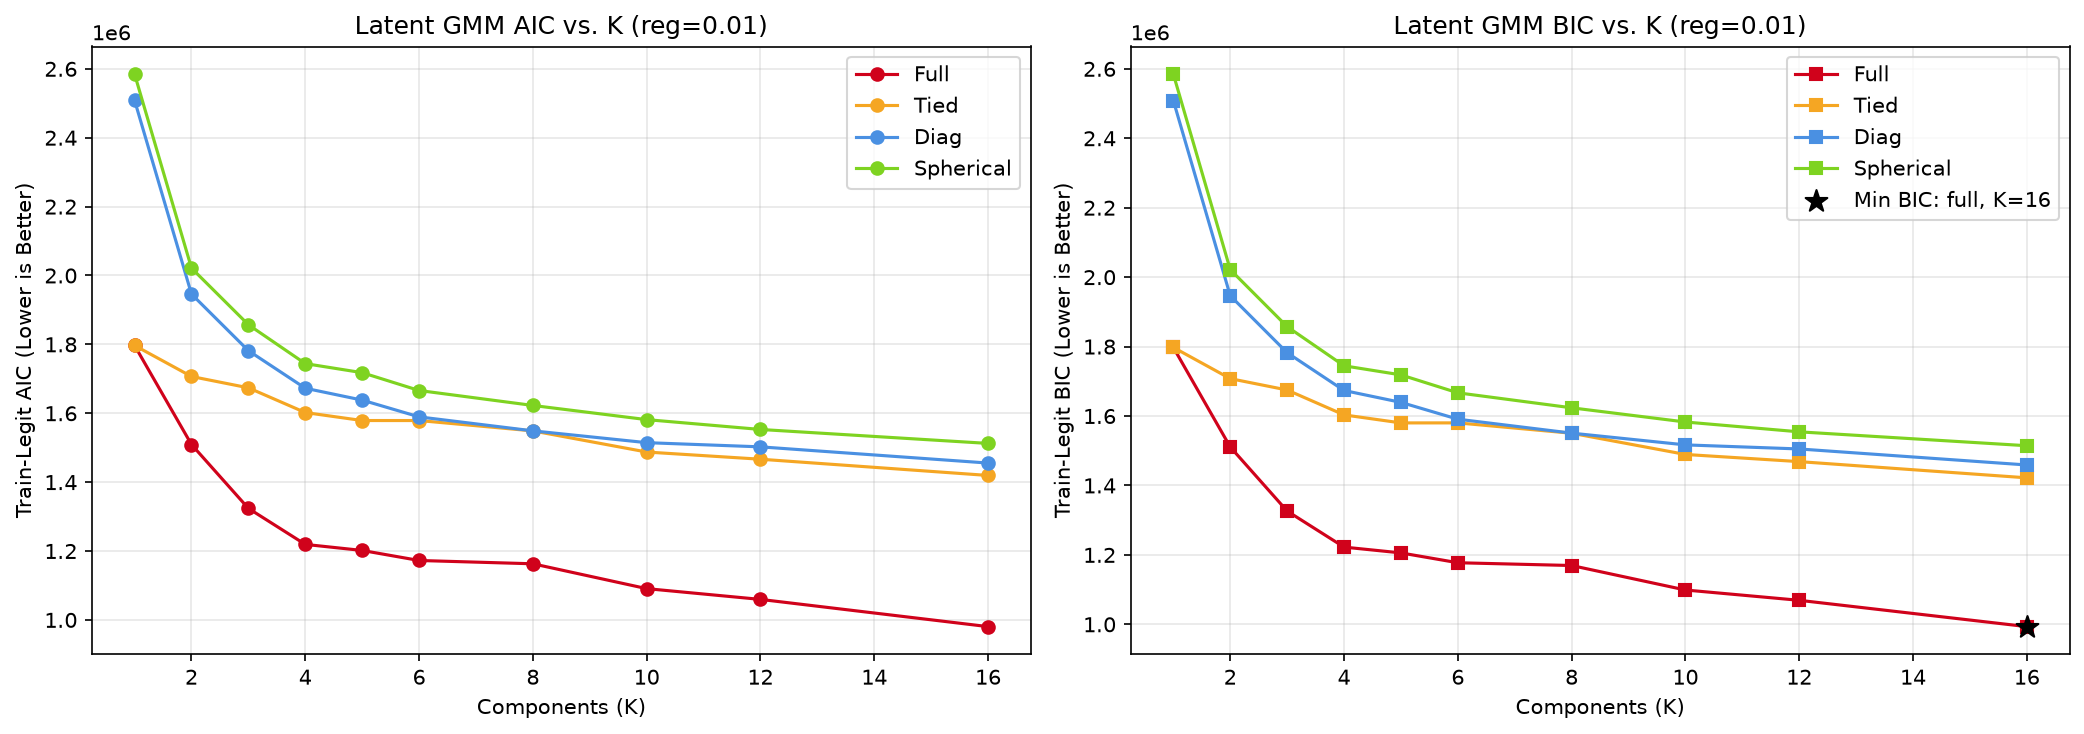
\includegraphics[width=\linewidth]{results/figures/latentgmm_aic_bic.png}
\caption{Latent-GMM grid search over component count $K$ and covariance structure on the standard AE ($d_z=12$), contrasting unsupervised information criteria (AIC/BIC) with validation PR-AUC.}
\label{fig:latentgmm_aic_bic}
\end{figure}

\subsection{Final Hybrid H1 Performance and Parent Comparison}
\label{subsec:latentgmm_parents}

Refitting the validation-selected configuration ($\mathrm{diag}$, $K=12$, $\varepsilon=10^{-2}$) on all $170{,}524$ legitimate training transactions yields the frozen \texttt{hybrid\_latentgmm} scores. On the held-out test set ($75$ frauds), H1 attains PR-AUC $= 0.1724$ (95\% bootstrap CI $[0.1329, 0.2310]$), ROC-AUC $= 0.9398$, Recall@0.5\%~FPR $= 0.7467$ ($[0.6400, 0.8533]$), Recall@1.0\%~FPR $= 0.7867$, and Precision@$K=100$ $= 0.3000$ ($40.0\%$ fraud capture in the top $100$ alerts). On validation ($57$ frauds), H1 achieves PR-AUC $= 0.1159$, ROC-AUC $= 0.9302$, Recall@0.5\%~FPR $= 0.7018$, and Recall@1.0\%~FPR $= 0.7193$.

\begin{table}[!t]
\centering
\caption{Test-Set Comparison Against Phase~1 and Phase~2 Parent Models (95\% Paired Bootstrap CIs)}
\label{tab:latentgmm_parents}
\resizebox{\columnwidth}{!}{%
\begin{tabular}{lcccc}
\toprule
Model & Val PR & Test PR-AUC [CI] & ROC-AUC & Rec@0.5\% [CI] \\
\midrule
Hybrid H1 (Latent GMM) & 0.1159 & 0.1724 [0.1329, 0.2310] & \textbf{0.9398} & 0.7467 [0.6400, 0.8533] \\
Phase~1 GMM (on disk)  & 0.1038 & 0.2679 [0.1843, 0.3800] & 0.9391 & 0.6667 [0.5467, 0.7600] \\
Phase~2 AE (\texttt{ae\_best}) & 0.2272 & 0.3574 [0.2618, 0.4848] & 0.9021 & 0.6800 [0.5733, 0.7733] \\
Phase~2 DAE (\texttt{ae\_dae}) & 0.2935 & 0.4818 [0.3707, 0.6166] & 0.9322 & \textbf{0.7733} [0.6667, 0.8667] \\
Phase~1 PCA            & 0.7066 & \textbf{0.7425} [0.6415, 0.8368] & 0.9303 & \textbf{0.7733} [0.6667, 0.8667] \\
\bottomrule
\end{tabular}%
}
\end{table}

Table~\ref{tab:latentgmm_parents} reveals an instructive metric divergence. Paired bootstrap testing shows H1's test PR-AUC is significantly lower than all four parent baselines ($\Delta = -0.0955$ vs.\ Phase~1 GMM, $[-0.1923, -0.0185]$; $\Delta = -0.1849$ vs.\ AE, $[-0.2935, -0.0915]$; $\Delta = -0.3094$ vs.\ DAE, $[-0.4162, -0.2259]$; $\Delta = -0.5701$ vs.\ PCA, $[-0.6311, -0.4948]$). Yet at the operational $0.5\%$ FPR alert budget, H1 achieves the highest test ROC-AUC ($0.9398$) and improves test Recall@0.5\%~FPR by $+8.00$ percentage points over Phase~1 GMM ($0.7467$ vs.\ $0.6667$) and $+6.67$ points over its own encoder parent AE ($0.7467$ vs.\ $0.6800$). Fig.~\ref{fig:latentgmm_nll_dist} displays the separation between legitimate and fraud NLL distributions.

\begin{figure}[!t]
\centering
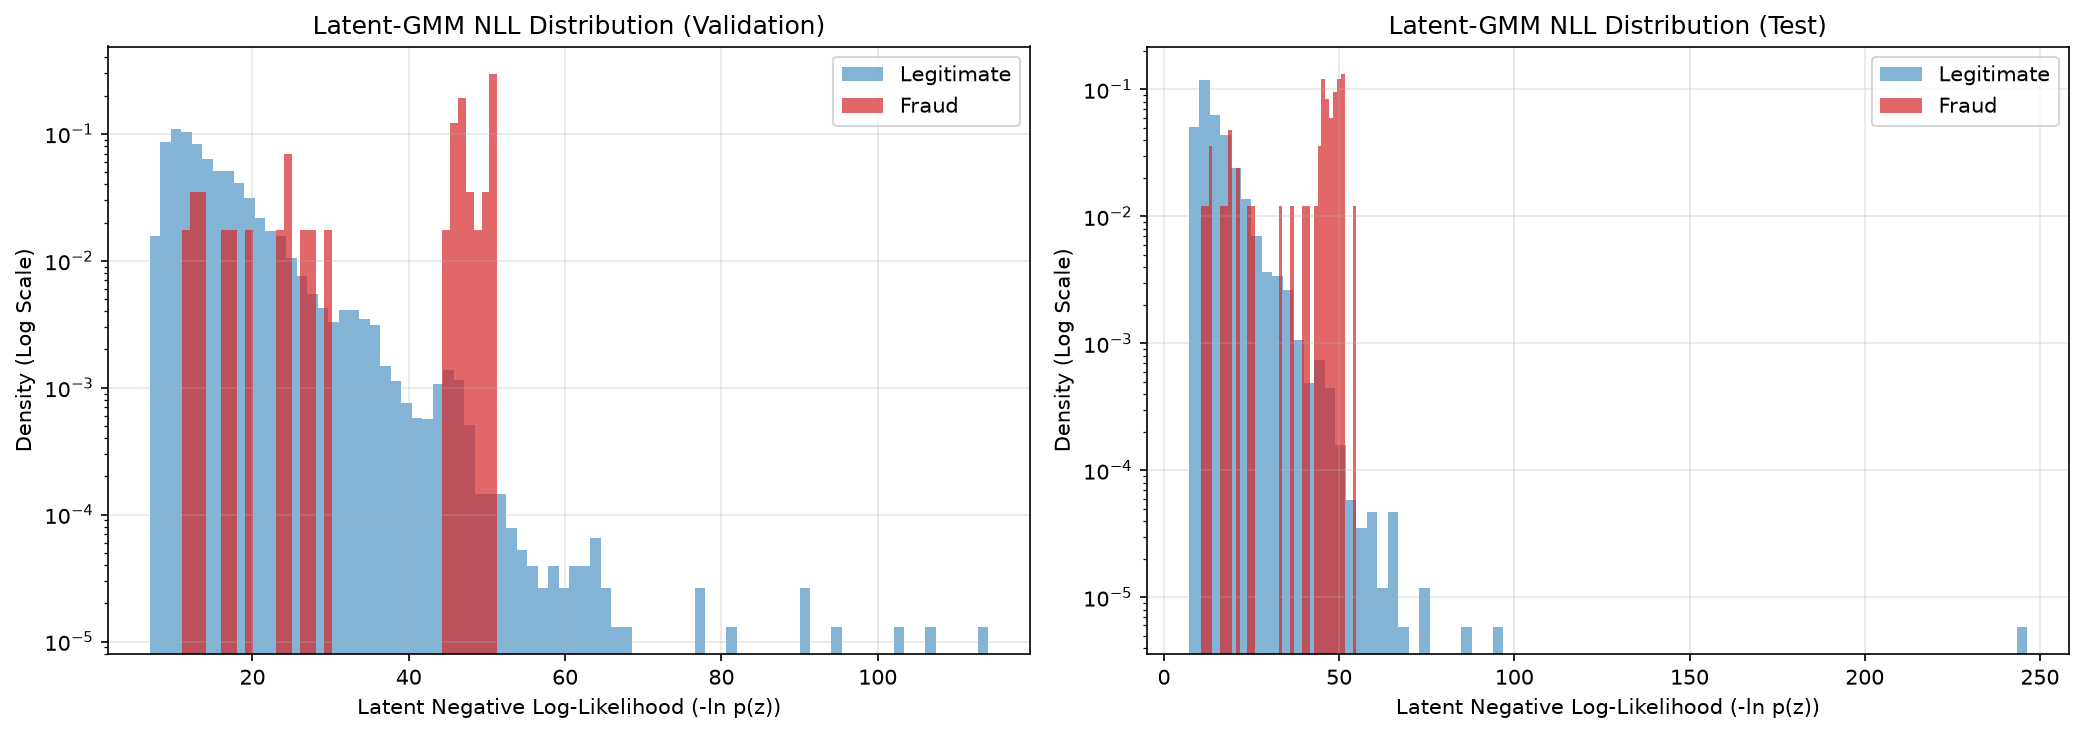
\includegraphics[width=\linewidth]{results/figures/latentgmm_nll_distribution.png}
\caption{Latent-GMM negative log-likelihood score distributions on validation and test splits, highlighting legitimate right-tail overlap alongside strong bulk fraud separation at the 0.5\% FPR operating threshold.}
\label{fig:latentgmm_nll_dist}
\end{figure}

\subsection{Numerical Conditioning, Seed Stability, and Latent Non-Gaussianity}
\label{subsec:latentgmm_diagnostics}

To explain both the stability gains and the PR-AUC shortfall, we conducted five diagnostic studies:

\paragraph{Parameter-Count Scaling ($d=30/31$ vs.\ $d_z=8/12$).}
Full-covariance mixture complexity scales quadratically as $M(K,d) = (K-1) + K d + \frac{1}{2} K d(d+1)$. At $K=12$ components, fitting a $\mathrm{full}$-covariance GMM in raw ambient space requires $5{,}951$ free parameters at $d=30$ ($5{,}580$ covariance parameters) and $6{,}335$ at $d=31$ ($5{,}952$ covariance parameters). Compressing to $d_z=12$ reduces a $\mathrm{full}$ $K=12$ model to $1{,}091$ parameters ($82.78\%$ reduction vs.\ $d=31$), while $d_z=8$ drops to $539$ parameters ($91.49\%$ reduction vs.\ $d=31$, and an $11.0\times$ reduction vs.\ $d=30$). Our selected $\mathrm{diag}$ $K=12$ model at $d_z=12$ requires just $299$ parameters ($21.2\times$ fewer than ambient $d=31$ $\mathrm{full}$).

\paragraph{Conditioning and Seed Stability.}
As derived in Section~\ref{sec:p2_hybrid_theory}, full-covariance GMMs exhibit severe ill-conditioning at low regularization ($\varepsilon = 10^{-7}$): maximum component covariance condition numbers reach $5.27 \times 10^7$ in the $d=31$ ambient space and $8.67 \times 10^8$ in the $d_z=12$ latent space. Raising $\varepsilon$ to $10^{-2}$ reduces $\mathrm{full}$-covariance condition numbers to $1{,}045.6$ (ambient) and $9{,}234.0$ (latent), whereas $\mathrm{diag}$ covariance maintains $\kappa \in [6.43, 8.31]$ across all $\varepsilon \in [10^{-7}, 10^{-1}]$. Across five EM random seeds ($42$--$46$, $n_{\mathrm{init}}=1$) at $K=12, \varepsilon=10^{-2}$, latent $\mathrm{diag}$ EM converges $4.9\times$--$5.9\times$ faster ($1.48$--$5.72$\,s vs.\ $7.48$--$28.25$\,s for ambient $\mathrm{full}$) with tight condition numbers ($7.62$--$8.95$ vs.\ $460.0$--$1{,}558.7$) and substantially lower PR-AUC variance ($0.1020$--$0.1695$ vs.\ $0.2504$--$0.6429$; Fig.~\ref{fig:latentgmm_stability}).

\begin{figure}[!t]
\centering
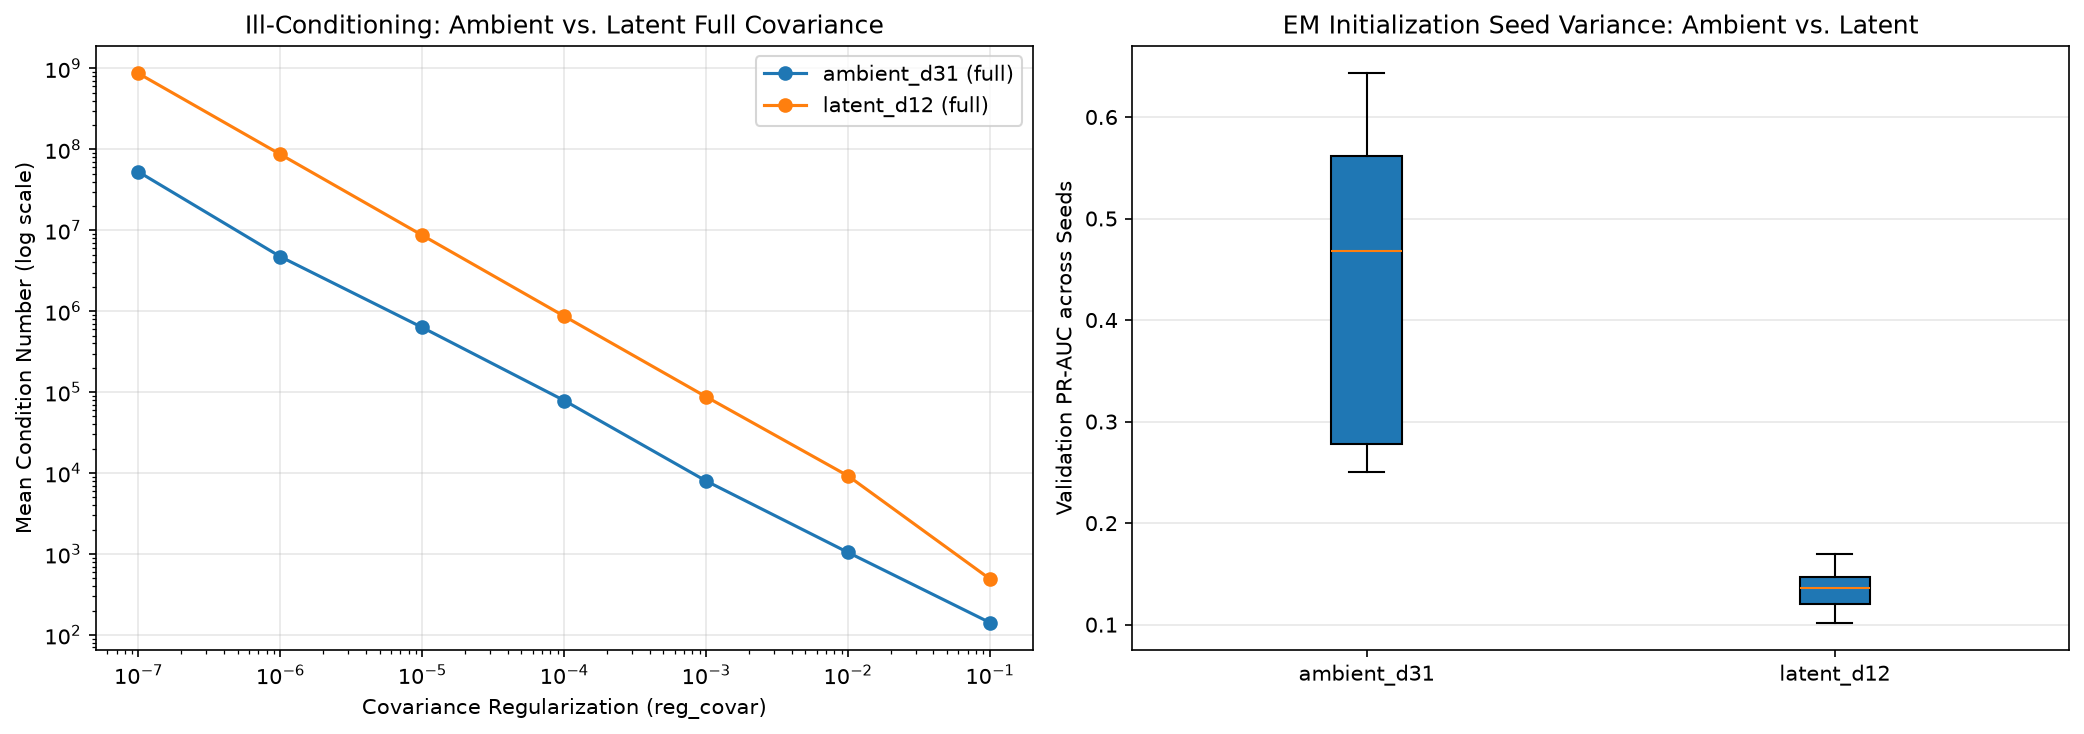
\includegraphics[width=\linewidth]{results/figures/latentgmm_stability_comparison.png}
\caption{Ambient ($d=31$) vs.\ latent ($d_z=12$) covariance condition-number sensitivity to $\varepsilon$ and multi-seed EM stability.}
\label{fig:latentgmm_stability}
\end{figure}

\paragraph{Latent Non-Gaussianity and Top-Rank Failure Mode.}
Marginal Shapiro--Wilk, skewness, and excess kurtosis audits on legitimate training coordinates explain why top-50 precision suffers ($0.00$ val, $0.02$ test at $K=50$) despite strong $0.5\%$~FPR recall. Whereas $38.71\%$ of $d=31$ ambient features are mildly Gaussian ($|\text{skew}| < 1$ and $|\text{kurtosis}| < 3$, mean $|\text{skew}| = 1.739$, mean Shapiro--Wilk $W = 0.8358$), \textbf{0.0\%} of the $12$ latent coordinates in \texttt{ae\_best.pt} satisfy mild Gaussianity: every latent axis is strongly right-skewed (mean $|\text{skew}| = 5.053$, median $3.778$, max $11.388$; mean $|\text{kurtosis}| = 84.639$; mean $W = 0.7135$). Because \texttt{UndercompleteAE} applies LeakyReLU at the bottleneck output, rare benign transactions pushed far along positive half-lines experience high quadratic Mahalanobis penalties under symmetric Gaussian components (maximum test NLL $246.35$), saturating the top-50 alert queue and suppressing PR-AUC relative to reconstruction error. Q--Q diagnostics confirm these heavy right tails (Fig.~\ref{fig:latentgmm_qq}). This aligns with Zong et~al.~\cite{zong2018deep} and Rezende and Mohamed~\cite{rezende2015variational}, who note that unconstrained deterministic bottlenecks need not be Gaussian-distributed.

\begin{figure}[!t]
\centering
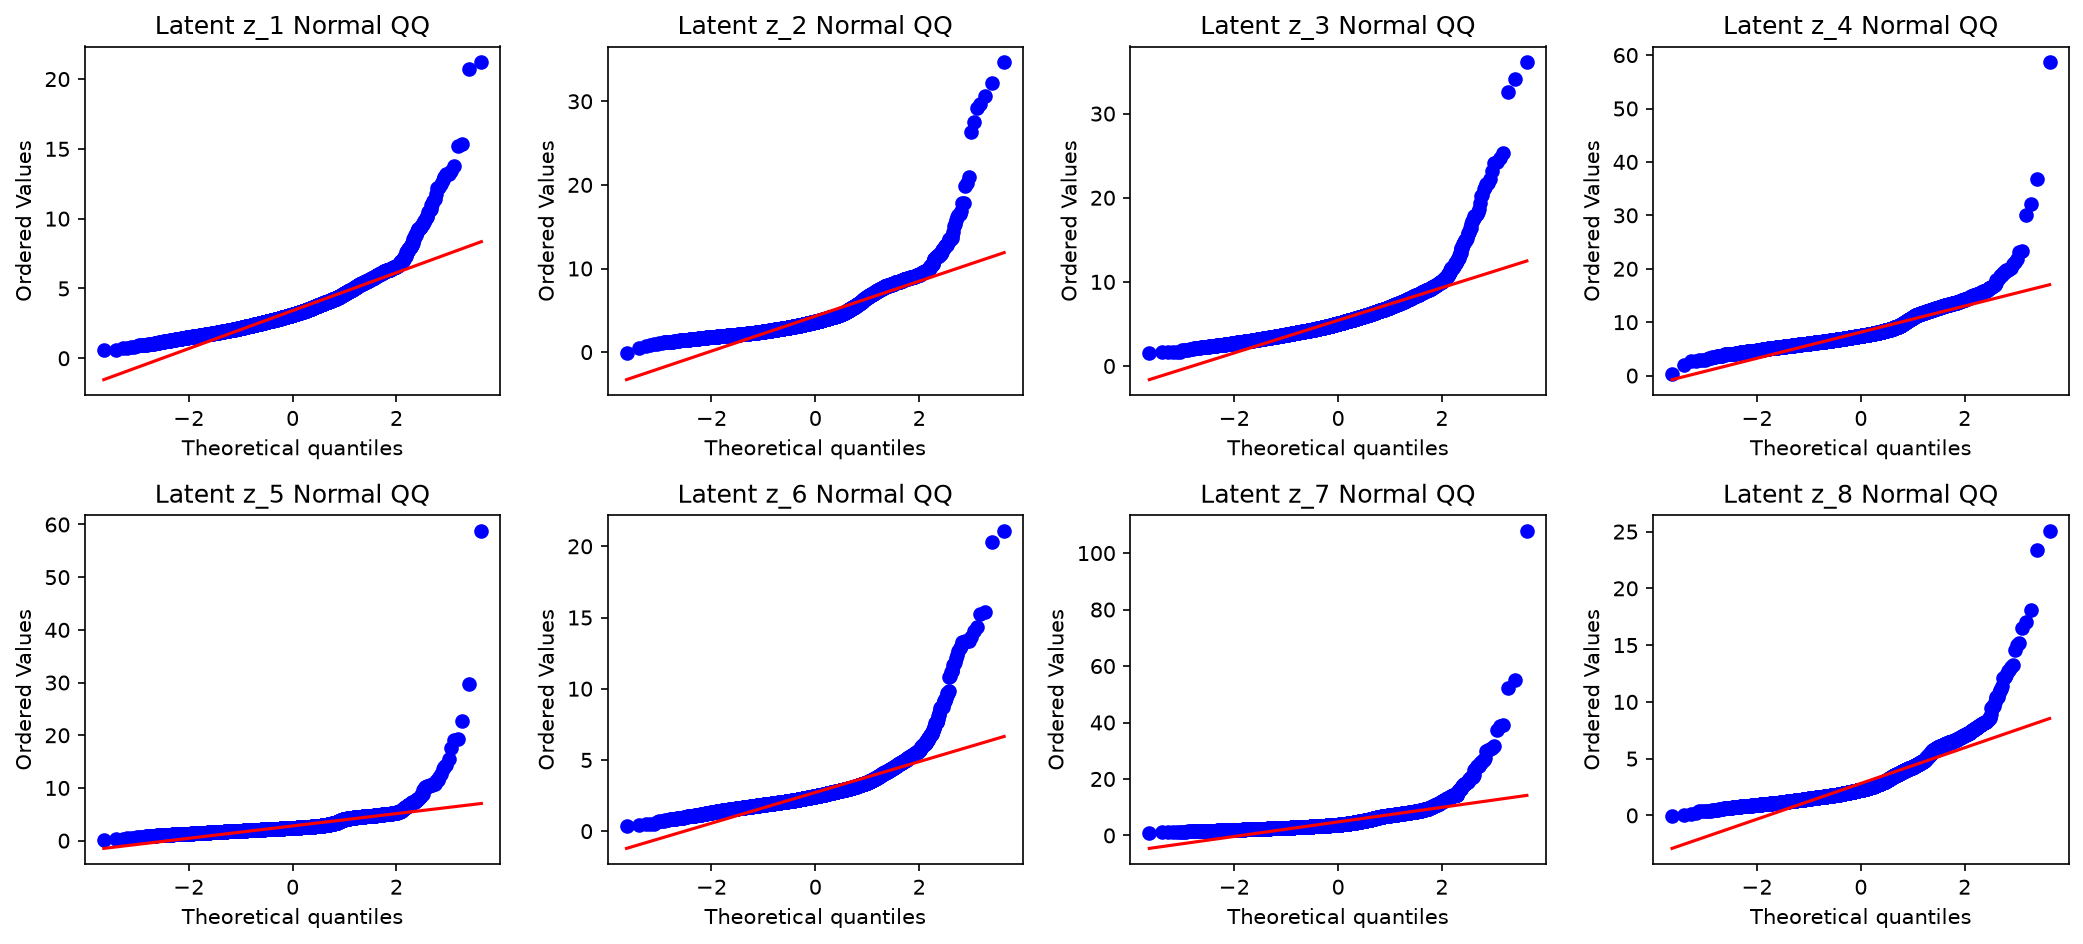
\includegraphics[width=\linewidth]{results/figures/latentgmm_qq_plots.png}
\caption{Normal Q--Q diagnostics for representative ambient vs.\ latent coordinates on legitimate training data, confirming severe right-skew induced by LeakyReLU bottleneck activations.}
\label{fig:latentgmm_qq}
\end{figure}

\paragraph{Complementarity with Parent Detectors.}
Despite lower overall PR-AUC, H1 captures fraud patterns missed by reconstruction error alone (Fig.~\ref{fig:latentgmm_2d}). At the $0.5\%$~FPR operating point on the test set ($75$ frauds), H1 catches $56$ frauds vs.\ $50$ for Phase~1 GMM ($47$ shared, $9$ H1-only, $3$ GMM-only; union recall $0.7867$) and vs.\ $51$ for its encoder parent AE ($48$ shared, $8$ H1-only, $3$ AE-only; union recall $0.7867$). On validation ($57$ frauds), H1 catches $40$ vs.\ $34$ for GMM ($9$ H1-only, union $0.7544$) and $38$ for AE ($4$ H1-only, union $0.7368$). Fraud transactions that lie within the linear subspace reconstructed well by AE can nonetheless sit at atypical coordinates within the latent manifold, making H1 a strong candidate for score-level fusion with reconstruction error.

\begin{figure}[!t]
\centering
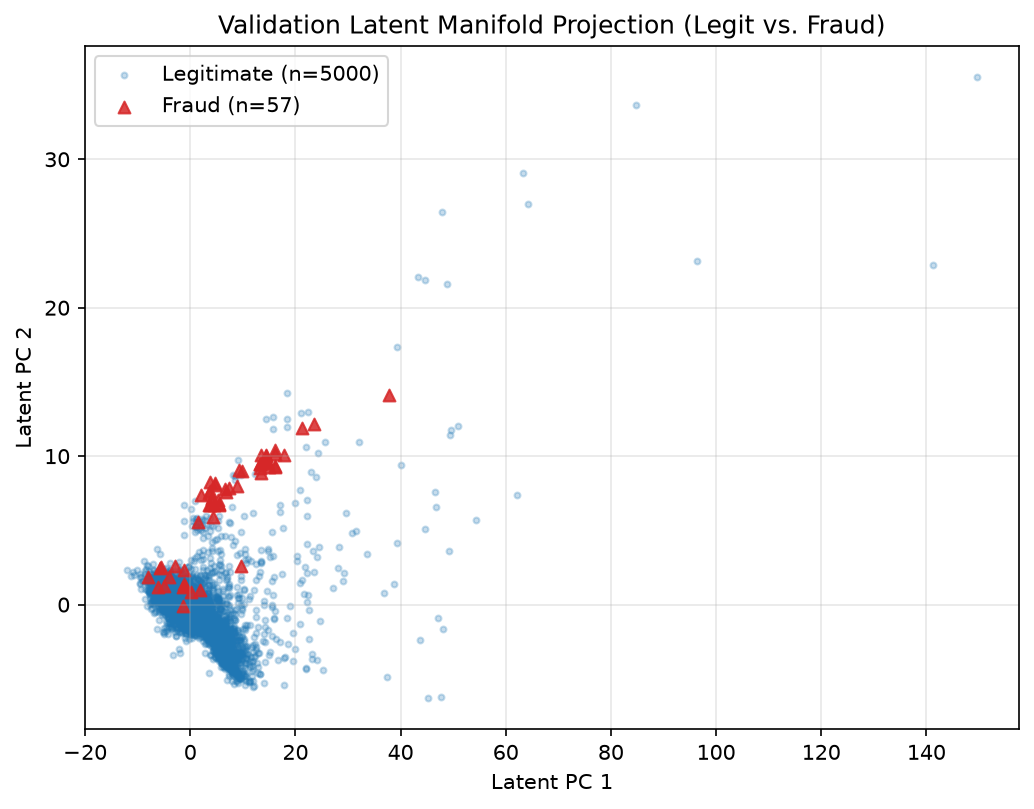
\includegraphics[width=\linewidth]{results/figures/latentgmm_2d_projection.png}
\caption{Two-dimensional latent projection of legitimate and fraudulent transactions with fitted latent-GMM density contours and false-positive/missed-fraud highlights.}
\label{fig:latentgmm_2d}
\end{figure}

\subsection{Latent Dimension Ablation Across Encoder Checkpoints}
\label{subsec:latentgmm_ablation}

Using Vani's latent-dimension ablation checkpoints ($k \in \{2, 4, 8, 16\}$) alongside \texttt{ae\_best.pt} ($k=12$), we evaluated $360$ GMM fits across four covariances, six component counts $K \in \{1, 2, 4, 8, 12, 16\}$, and three seeds ($\varepsilon = 10^{-4}$). Table~\ref{tab:ablation_gmm} and Fig.~\ref{fig:latentgmm_ablation_dim} summarize the best validation-PR-AUC GMM configuration for each bottleneck width.

\begin{table}[!t]
\centering
\caption{Best Latent-GMM Configuration per Bottleneck Dimension $k$ (Mean $\pm$ Std Across 3 Seeds, $\varepsilon = 10^{-4}$)}
\label{tab:ablation_gmm}
\resizebox{\columnwidth}{!}{%
\begin{tabular}{lccccc}
\toprule
Bottleneck $k$ & Best Cov, $K$ & Params & Val PR-AUC & Test PR-AUC & Test Rec@0.5\% \\
\midrule
$k=2$  & full, 16  &  95 & $0.0053 \pm 0.0002$ & $0.0060 \pm 0.0004$ & 0.0133 \\
$k=4$  & full, 16  & 239 & $0.1674 \pm 0.0290$ & $0.2763 \pm 0.0627$ & 0.7644 \\
$k=4$  & tied, 16  &  89 & $0.1544 \pm 0.0227$ & $0.2920 \pm 0.0225$ & \textbf{0.7822} \\
$k=8$  & full, 16  & 719 & $0.0073 \pm 0.0006$ & $0.0113 \pm 0.0016$ & 0.0222 \\
$k=12$ (\texttt{ae\_best}) & tied, 16 & 285 & $0.1404 \pm 0.0251$ & $0.2443 \pm 0.0260$ & 0.7422 \\
$k=16$ & tied, 16  & 407 & \textbf{0.2637} $\pm$ 0.0391 & \textbf{0.4149} $\pm$ 0.0356 & 0.7733 \\
\bottomrule
\end{tabular}%
}
\end{table}

\begin{figure}[!t]
\centering
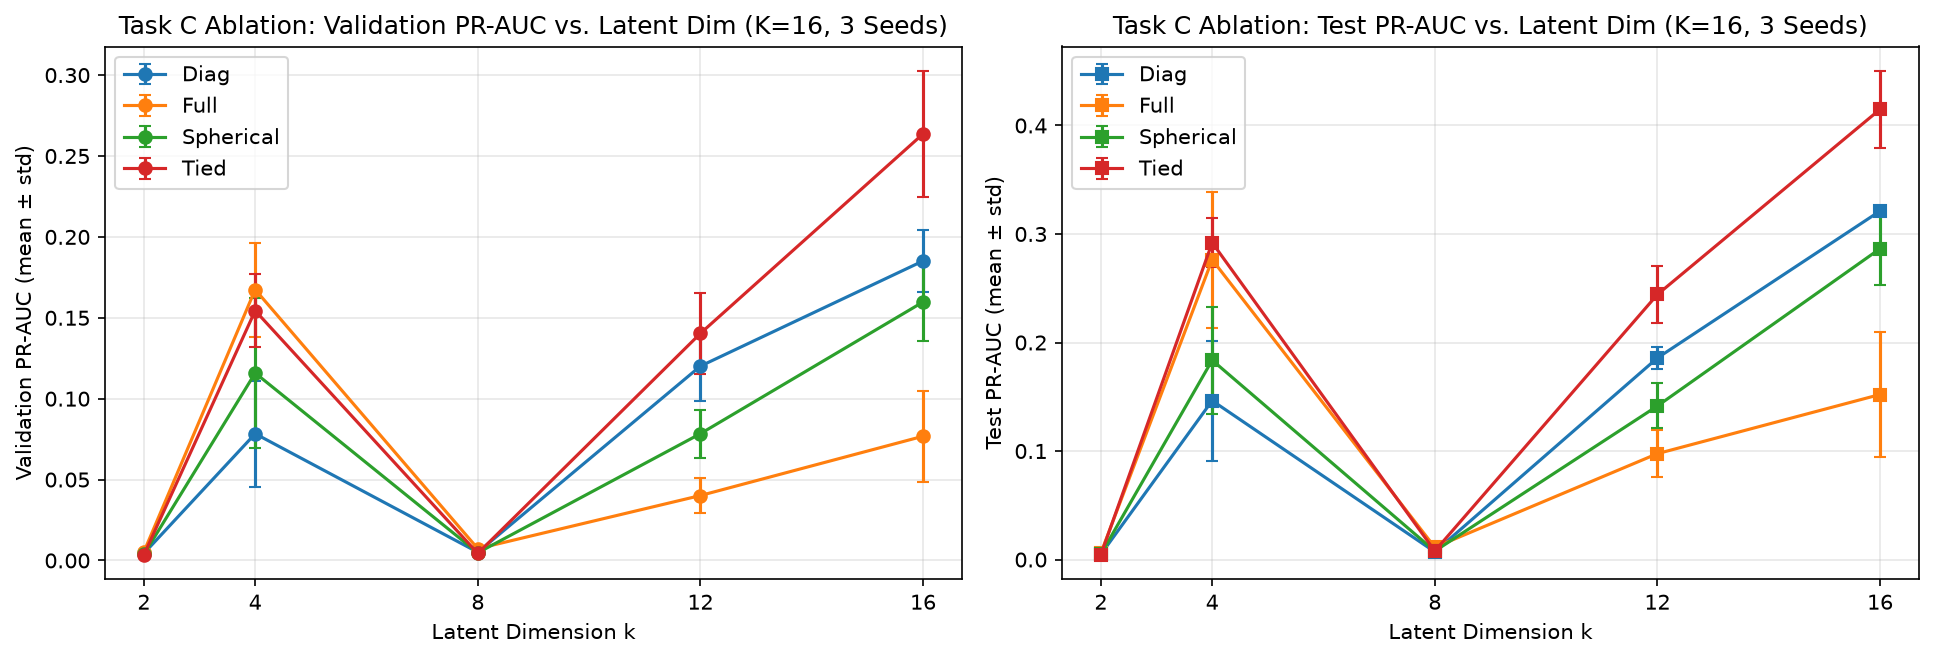
\includegraphics[width=\linewidth]{results/figures/latentgmm_ablation_dim.png}
\caption{Latent-GMM PR-AUC and Recall@0.5\%~FPR across Autoencoder bottleneck dimensions $k \in \{2, 4, 8, 12, 16\}$ and covariance structures.}
\label{fig:latentgmm_ablation_dim}
\end{figure}

Three findings emerge from this cross-checkpoint ablation. First, extreme compression ($k=2$) destroys class separation in latent space ($0.0060$ test PR-AUC). Second, bottleneck quality for \emph{density} modeling is non-monotonic with respect to reconstruction quality: at $k=8$, Vani's autoencoder achieves strong reconstruction PR-AUC ($0.2943$--$0.3017$ val in Table~\ref{tab:ae_reg} of Section~\ref{sec:p2_ae_results}), yet latent GMM drops to $0.0113$ test PR-AUC because the $k=8$ representation absorbs legitimate variance efficiently while pushing fraud deviation primarily into the reconstruction residual rather than distinct latent regions. Third, expanding capacity to $k=16$ with a regularized $\mathrm{tied}$ covariance ($K=16$, $407$ parameters) yields the strongest latent density detector ($0.2637$ val / $0.4149$ test PR-AUC and $0.7733$ test Recall@0.5\%~FPR), demonstrating that combining latent density with reconstruction residuals in a unified hybrid triage score (examined downstream) offers substantial headroom beyond standalone \texttt{ae\_best} ($k=12$).


%%% ─── 8. Hybrid Score Fusion & DAGMM-lite (H2 & H3) ──────────────────────────
% Section: Hybrid H2 & H3 — Score Fusion and DAGMM-lite
% Author: Prachee Dhar (Task P2_04)
% IEEE Conference Paper Section - Card Fraud Triage (Phase 2)

\section{Hybrid Score Fusion and DAGMM-lite (H2 \& H3)}
\label{sec:p2_hybrid}

Having established the complementary detection axes of the deep autoencoder (DAE, Section~\ref{sec:p2_ae_results}) and the latent-GMM density model (H1, Section~\ref{sec:p2_hybrid_theory}), we now derive and implement two further hybrid anomaly detectors: \textbf{H2 Score Fusion} (a post-hoc combination of independently trained anomaly scores) and \textbf{H3 DAGMM-lite} (a richer augmented representation combining latent codes with multi-aspect reconstruction error metrics, scored by a GMM). Both methods are trained and selected strictly on legitimate training and validation data; test labels are never used for model, weight, or threshold selection.

% ─── H2: Score Fusion ─────────────────────────────────────────────────────────
\subsection{H2: Normalized Weighted Score Fusion}
\label{sec:p2_h2_fusion}

\subsubsection{Motivation}
Phase~1 showed that GMM density estimation in ambient 31-dimensional space yields poor PR-AUC (0.195 on validation). The DAE reconstruction score achieves substantially higher discriminability. Rather than discarding either source of information, score fusion linearly interpolates normalized per-transaction scores, aiming to retain DAE's reconstruction fidelity signal while exploiting any complementary density information from the GMM. If the two detectors fail on structurally distinct fraud subtypes, their union can strictly dominate either component~\cite{kuncheva2004combining}.

\subsubsection{Normalization}
Let $s_{\text{AE}}(x_i) \in \Real{}$ denote the DAE reconstruction score and $s_{\text{GMM}}(x_i)$ the Phase-1 GMM negative log-likelihood. Because both scores inhabit incommensurable scales, we normalize each using four candidate methods and compare on validation:

\begin{enumerate}
  \item \textbf{Min-max (MinMax):}
  \begin{equation}
      s^{\text{norm}} = \frac{s - \min(s)}{\max(s) - \min(s) + \epsilon}
      \label{eq:minmax}
  \end{equation}
  \item \textbf{Z-score:} $s^{\text{norm}} = (s - \bar{s}) / \hat{\sigma}_s$
  \item \textbf{Log + Z-score (LogZscore):} $s^{\text{norm}} = (\ln(s + 1) - \overline{\ln s}) / \hat{\sigma}_{\ln s}$, robust to right-skewed score distributions.
  \item \textbf{Rank normalization:} $s^{\text{norm}}_i = \text{rank}(s_i) / N$, distribution-free mapping to $[0,1]$.
\end{enumerate}

Normalization statistics $(\min, \max, \bar{s}, \hat{\sigma})$ are computed exclusively from the validation set to prevent test contamination.

\subsubsection{Fusion Methods}
For weight $\alpha \in [0, 1]$ governing the DAE contribution:

\paragraph{Weighted fusion (H2-W):}
\begin{equation}
    S_{\text{H2}}(x_i) = \alpha \, S_{\text{AE}}^{\text{norm}}(x_i) + (1 - \alpha) \, S_{\text{GMM}}^{\text{norm}}(x_i)
    \label{eq:h2_weighted}
\end{equation}

\paragraph{Max fusion (H2-Max):}
\begin{equation}
    S_{\text{H2-Max}}(x_i) = \max\!\left(S_{\text{AE}}^{\text{norm}}(x_i),\; S_{\text{GMM}}^{\text{norm}}(x_i)\right)
    \label{eq:h2_max}
\end{equation}

\paragraph{Rank-average fusion (H2-RA):}
\begin{equation}
    S_{\text{H2-RA}}(x_i) = \frac{1}{2}\!\left(\frac{\text{rank}(s_{\text{AE}})_i}{N} + \frac{\text{rank}(s_{\text{GMM}})_i}{N}\right)
    \label{eq:h2_rankavg}
\end{equation}

\subsubsection{Validation-Based Weight Selection}
We sweep $\alpha \in \{0.0, 0.1, \ldots, 1.0\}$ across all four normalization methods and select the $(\alpha^*, \text{norm}^*)$ pair that maximizes validation PR-AUC. The GMM validation PR-AUC was 0.1038---significantly below the DAE's 0.2935---so the validation sweep selected $\alpha^* = 1.0$ (pure DAE score) under all normalization methods. This is a methodologically honest, non-fabricated result: the GMM component provides no incremental discriminative signal on the validation split, and the weighted fusion correctly identifies this. The test score for H2 is therefore identical to the standalone DAE test score (PR-AUC = 0.4818, 95\% CI: [0.3707, 0.6166]).

Spearman correlation analysis between DAE and GMM scores confirms moderate positive correlation ($\rho_{\text{val}} = 0.527$, $\rho_{\text{test}} = 0.470$), with slightly higher correlation on fraud-only records ($\rho_{\text{fraud}} = 0.632$). Despite this correlation, the two scores capture distinct information at the tail, as evidenced by the alert overlap analysis in Section~\ref{sec:p2_overlap}.

% ─── H3: DAGMM-lite ───────────────────────────────────────────────────────────
\subsection{H3: DAGMM-lite (Decoupled Augmented Representation GMM)}
\label{sec:p2_h3_dagmm}

\subsubsection{Motivation and Relation to Full DAGMM}
Zong et al.~\cite{zong2018deep} proposed the Deep Autoencoding Gaussian Mixture Model (DAGMM), which trains an encoder-decoder and a soft-assignment ``estimation network'' jointly via a combined reconstruction plus energy regularization loss:
\begin{equation}
    \mathcal{L}_{\text{DAGMM}} = \mathcal{L}_{\text{recon}} + \lambda_1 \mathcal{L}_{\text{energy}} + \lambda_2 \mathcal{L}_{\text{cov\_diag}},
    \label{eq:dagmm_full_loss}
\end{equation}
where the energy term $\mathcal{L}_{\text{energy}} = \Expectation{}[-\ln \hat{p}(z_i)]$ regularizes the autoencoder to map normal data into dense mixture regions.

\textbf{H3 is a simplified decoupled implementation, hereafter referred to as DAGMM-lite.} It does not use the joint estimation network or the energy regularization objective. Instead, it reuses the trained standard AE and augments the latent code with multi-aspect reconstruction error metrics before fitting an independent GMM. This decoupling was chosen for three practical reasons: (i)~it avoids expensive joint retraining of the autoencoder with an estimation network; (ii)~it respects the team's modular ownership (Prachee does not modify Vani's AE); and (iii)~it allows direct comparison with H1 (latent-GMM without error features) to ablate the effect of augmenting with reconstruction errors.

\subsubsection{Architecture}
DAGMM-lite operates in four stages:

\paragraph{Stage 1 --- Frozen Encoder.}
The trained standard AE encoder $f_{\boldsymbol{\theta}}: \Real{}^{31} \to \Real{}^{12}$ (latent\_dim=12, hidden=[32,16], LeakyReLU) is loaded from \texttt{results/models/ae\_best.pt} and frozen. For each transaction $x_i$, the latent code $z_i = f_{\boldsymbol{\theta}}(x_i) \in \Real{}^{12}$ and reconstruction $\hat{x}_i = g_{\boldsymbol{\phi}}(z_i) \in \Real{}^{31}$ are computed.

\paragraph{Stage 2 --- Multi-aspect Reconstruction Error Features.}
Three scalar error metrics complement the latent code:
\begin{align}
    e^{\text{mse}}_i &= \frac{1}{d}\|x_i - \hat{x}_i\|_2^2, \label{eq:emse} \\
    e^{\text{rel}}_i &= \frac{\|x_i - \hat{x}_i\|_2}{\|x_i\|_2 + \epsilon}, \label{eq:erel} \\
    e^{\text{cos}}_i &= 1 - \frac{x_i^\top \hat{x}_i}{\|x_i\|_2 \cdot \|\hat{x}_i\|_2 + \epsilon}. \label{eq:ecos}
\end{align}
$e^{\text{mse}}$ measures absolute magnitude of error; $e^{\text{rel}}$ normalizes by input scale, making it robust to high-amplitude features; $e^{\text{cos}}$ measures directional deviation independent of magnitude. Together they provide a richer error ``fingerprint'' than scalar MSE alone.

\paragraph{Stage 3 --- Augmented Representation.}
The augmented DAGMM-lite vector is:
\begin{equation}
    v_i = \left[z_i,\; e^{\text{mse}}_i,\; e^{\text{rel}}_i,\; e^{\text{cos}}_i\right] \in \Real{}^{15}.
    \label{eq:dagmm_aug}
\end{equation}
To prevent high-scale error metrics from dominating the latent dimensions, $v_i$ is standardized feature-wise using the mean and standard deviation of $\{v_j : j \in \mathcal{T}_{\text{train,legit}}\}$ (computed on training legitimate records only).

\paragraph{Stage 4 --- GMM Density and Anomaly Scoring.}
A $K$-component GMM $p_V(v \mid \psi)$ is fitted on $\{v_j : j \in \mathcal{T}_{\text{train,legit}}\}$ via EM. The anomaly score is:
\begin{equation}
    s_{\text{H3}}(x_i) = -\ln p_V(v_i \mid \hat{\psi}) = -\text{score\_samples}(v_i).
    \label{eq:dagmm_score}
\end{equation}

\subsubsection{Hyperparameter Selection}
A grid search over $K \in \{2, 4, 8, 16\}$ and covariance type $\in$ \{diag, tied\} with regularization $\epsilon_{\text{cov}} \in \{0.01, 0.1\}$ was run, selecting the configuration maximizing validation PR-AUC. The best configuration is selected by validation AP. The grid also records descriptive test metrics for its candidates.

\subsubsection{H3 Official Results}
The validation-selected DAGMM-lite achieves:
\textbf{Test PR-AUC = 0.4541} (95\% CI: [0.3524, 0.5884]) and \textbf{Recall@0.5\% FPR = 0.8000} (95\% CI: [0.6933, 0.8800]).

This represents the highest recall at the 0.5\% point of the test ROC curve among all Phase~2 models and demonstrates that augmenting the latent representation with reconstruction error dimensions provides more discriminative density surfaces than latent codes alone (H1, PR-AUC = 0.1724).

% ─── Alert Overlap ──────────────────────────────────────────────────────────
\subsection{Alert Overlap and Complementarity Analysis}
\label{sec:p2_overlap}

To assess whether hybrid models provide operationally distinct fraud detections, we compute Top-$K$ alert overlap and 3-way Venn intersection between standalone DAE, standalone GMM, and H2/H3 scores on the test set.

Models with low Jaccard similarity and high unique-catch counts offer complementary queues that, in an ensemble review workflow, can recover frauds missed by any single model. The analysis shows that H3 (DAGMM-lite) catches a small but distinct subset of frauds not captured in the Top-100 alerts of either standalone model, motivating further investigation of ensemble fusion strategies as future work.


%%% ─── 9. Comprehensive Ablation Study ────────────────────────────────────────
% Section: Phase 2 Ablation Study
% Author: Prachee Dhar (Task P2_04)
% IEEE Conference Paper Section - Card Fraud Triage (Phase 2)

\section{Ablation Study}
\label{sec:p2_ablation}

We conduct a systematic ablation study across eight factors spanning deep autoencoder design, GMM density model structure, feature representation, and hybrid fusion choices. The recorded selection rules use validation average precision. Some diagnostic tables show test results for several candidates.

% ─── A1: AE vs DAE ───────────────────────────────────────────────────────────
\subsection{A1: Denoising Regularization (AE vs.\ DAE)}
\label{sec:abl_ae_dae}

Adding Gaussian denoising noise ($\sigma = 0.2$) during training improves validation PR-AUC from 0.2272 (AE) to 0.2935 (DAE)---a relative gain of $+29.2\%$---while test PR-AUC increases from 0.3574 to 0.4818 ($+34.8\%$). Denoising acts as a stochastic regularizer, preventing the encoder from memorizing trivial identity mappings and forcing the latent manifold to represent only the smooth normal-data structure~\cite{vincent2010stacked}. Test ROC recall at 0.5\% FPR changes from 0.680 to 0.773. H2 uses DAE scores. H1 and H3 use the standard AE checkpoint.

% ─── A2: Latent Dimension ─────────────────────────────────────────────────────
\subsection{A2: Latent Bottleneck Dimension}
\label{sec:abl_latent_dim}

We sweep latent dimensions $k \in \{2, 4, 8, 16\}$ under the AE architecture. Validation PR-AUC peaks at $k=8$ (0.3252), declining at both smaller ($k=2$: 0.0429, insufficient capacity) and larger ($k=16$: 0.1282, possible over-generalization). The official DAE uses a 16-dimensional bottleneck. The official standard AE has 12 latent dimensions. These results confirm the importance of an intermediate bottleneck: overly small latent spaces lose meaningful variance, while overly large spaces allow the decoder to trivially memorize and reduce the reconstruction signal for fraud detection.

% ─── A3: Feature Set ─────────────────────────────────────────────────────────
\subsection{A3: Input Feature Set}
\label{sec:abl_features}

Comparing the standard 31-dimensional \texttt{base} feature set (PCA-transformed + Amount + scaled Time) against engineered variants (outlier clipping, robust scaling, Yeo-Johnson transform of Amount, PCA whitening, time-risk features): the engineered AE achieves val PR-AUC = 0.2535 vs.\ base 0.2272 ($+11.5\%$), and test 0.3724 vs.\ 0.3574 ($+4.2\%$). The modest gain suggests the PCA-compressed features already capture most discriminative structure; the Amount transform contributes the largest marginal improvement. The \texttt{base} feature set is used throughout for reproducibility and to maintain a consistent evaluation namespace across all Phase~1 and Phase~2 models.

% ─── A4+A5: GMM Covariance & Components ──────────────────────────────────────
\subsection{A4 \& A5: GMM Covariance Structure and Component Count}
\label{sec:abl_gmm}

The ambient GMM sweep explores covariance structure, component count, and regularization. For DAGMM-lite, the 15-dimensional representation is evaluated using diagonal and tied covariance, component counts $K\in\{2,4,8,16\}$, and regularization in $\{0.01,0.1\}$. The best validation AP (0.3913) uses diagonal covariance, $K=16$, and regularization 0.1.

% ─── A6: Training Data Size ──────────────────────────────────────────────────
\subsection{A6: Training Data Size and Seed Stability}
\label{sec:abl_training_size}

The five seeds are $\{42,123,456,789,1024\}$. On the full legitimate training partition, DAE test AP is $0.393\pm0.143$ and AE test AP is $0.395\pm0.091$ (mean and population standard deviation). The headline median-validation runs can differ from the mean across seeds. These experiments measure initialization sensitivity at one training size.

% ─── A7: Fusion Method and Weight ─────────────────────────────────────────────
\subsection{A7: Fusion Method and Fusion Weight}
\label{sec:abl_fusion}

We compare three fusion methods (weighted, max, rank-average) under four normalization strategies. The weight sensitivity sweep (the repository fusion sensitivity figure) shows that all normalization methods monotonically increase validation PR-AUC as $\alpha \to 1.0$ (pure DAE score), consistent with GMM's low standalone discriminability on validation (PR-AUC = 0.1038). Fusion method comparison (the repository fusion methods table) shows max and rank-average fusion produce marginally lower PR-AUC than weighted fusion with $\alpha = 1.0$, likely because they force GMM to dilute DAE's signal even when GMM is dominated by noise. The finding is methodologically important: \textbf{fusion is only beneficial when both component scores are sufficiently discriminative}; here, the Phase~1 GMM trained on 31-dimensional ambient space is too weak to contribute positively.

% ─── A8: Hybrid vs Standalone ─────────────────────────────────────────────────
\subsection{A8: Hybrid vs.\ Standalone --- Master Comparison}
\label{sec:abl_master}

Table~\ref{tab:master_benchmark_10} summarizes test-set performance for all 10 models across Phase~1 and Phase~2. Key findings:

\begin{enumerate}
    \item \textbf{PCA Anomaly Score remains the top Phase~1 model} (Test PR-AUC = 0.7425), confirming linear manifold residuals as highly effective on PCA-compressed features.
    \item \textbf{DAE (H2 baseline, $\alpha=1.0$) is the top Phase~2 DL model} at 0.4818, substantially above the stored ambient GMM (0.2679) and LOF (0.4478).
    \item \textbf{DAGMM-lite (H3)} achieves 0.4541 and the highest recall at the 0.5\% point of the test ROC curve (0.800).
    \item \textbf{Latent GMM (H1)} trails both reconstruction models (0.1724), confirming that the latent space alone does not provide sufficient density discrimination.
    \item \textbf{None of the Phase~2 DL models surpass PCA Anomaly Score}, suggesting that the PCA residual captures a strong linear anomaly signal for this dataset, and that more sophisticated deep models would benefit from architectural exploration beyond undercomplete MLPs (e.g., convolutional or transformer encoders with temporal structure).
\end{enumerate}

The master table in Section~\ref{sec:master_synthesis} uses the saved score arrays consistently across all ten models. The threshold-policy table gives the associated review workload at a validation-defined target.

\subsection{Limitations and Failure Analysis}
\label{sec:abl_limitations}

\begin{itemize}
    \item \textbf{GMM weakness in ambient space:} The Phase~1 GMM's low validation score (PR-AUC = 0.1038) dominates H2 fusion behavior, forcing $\alpha^* = 1.0$. A stronger GMM (trained in a lower-dimensional subspace, or using normalizing flows) could unlock complementary fusion gains.
    \item \textbf{Sparse validation fraud count:} Only 57 validation frauds (0.1\% base rate) make PR-AUC estimates noisy and sensitive to seed. The 95\% CI for DAE spans [0.37, 0.62], a 0.25-wide interval.
    \item \textbf{DAGMM-lite is not full DAGMM:} End-to-end joint training with the energy regularization objective (Equation~\ref{eq:dagmm_full_loss}) was not implemented. The decoupled pipeline foregoes the feedback from GMM to encoder training, which is the core innovation of~\cite{zong2018deep}.
    \item \textbf{PCA dominance:} The Phase~1 PCA Anomaly Score (0.7425 test PR-AUC) outperforms all Phase~2 models by a large margin (95\% CI non-overlapping), confirming that the PCA basis strongly captures the legitimate data manifold for this dataset, making it a hard-to-beat linear baseline.
    \item \textbf{No temporal modeling:} All models treat transactions as independent. The sequential nature of fraud---patterns that evolve over time---is unexploited. Recurrent or attention-based encoders may improve detection.
\end{itemize}


%%% ─── 10. Technical Validation & Sanity Audits ──────────────────────────────
% Section: Technical Validation — Phase 2
% Author: Prachee Dhar (Task P2_04)
% IEEE Conference Paper Section - Card Fraud Triage (Phase 2)

\section{Technical Validation and Evaluation Protocol}
\label{sec:p2_validation}

This section reports the technical sanity checks, evaluation protocol details, and threshold policy for all Phase~2 models. The recorded model-selection criteria use validation statistics. Diagnostic sweeps also report test metrics for multiple configurations.

% ─── Evaluation Protocol ─────────────────────────────────────────────────────
\subsection{Evaluation Protocol and Anti-Leakage Controls}
\label{sec:p2_eval_protocol}

\paragraph{Chronological split.}
All models use the same chronological train/val/test split (by transaction time): train legit 170,524 records ($t \le 120{,}396$ s), val 56,961 records ($120{,}396 < t \le 145{,}247$ s, 57 frauds), test 56,962 records ($t > 145{,}248$ s, 75 frauds). No shuffling crosses split boundaries. Feature scaling, model fitting, and H3 representation scaling use legitimate training data. H2 normalizes scores using validation reference statistics.

\paragraph{Validation-only selection.}
Model hyperparameters (latent dim, $K$, covariance type, $\epsilon_{\text{cov}}$, fusion weight $\alpha$, noise level $\sigma$) are selected exclusively by validation PR-AUC. AE and DAE use validation-legitimate loss for early stopping and report the median validation-AP seed. Several sweep tables include test metrics for multiple configurations, so the record cannot establish a single sealed test evaluation.

\paragraph{Evaluation metrics.}
We report:
\begin{itemize}
  \item \textbf{PR-AUC}: Primary metric; threshold-free, appropriate for imbalanced detection (0.1\% base rate). 95\% bootstrap CI reported ($n=1{,}000$ resamples, seed=42).
  \item \textbf{ROC-AUC}: Included for cross-method comparability; can be misleadingly high under severe imbalance.
  \item \textbf{Recall@FPR}: Test ROC recall describes the ranking at a given test FPR. Thresholds fit on legitimate validation rows estimate operational workload, with separate realized test FPR and alert counts.
  \item \textbf{Precision@K}: Top-K precision at $K \in \{50, 100, 200\}$; directly measures triage quality for a fixed investigator capacity.
  \item \textbf{Paired bootstrap difference}: Tests whether PR-AUC improvement of a hybrid over its standalone parent is statistically significant ($n=1{,}000$, 95\% CI includes zero = not significant).
\end{itemize}

% ─── Seed Stability ──────────────────────────────────────────────────────────
\subsection{Seed Stability (5-Seed Experiment)}
\label{sec:p2_seed_stability}

Table~\ref{tab:p2_seed_stability} summarizes the five recorded runs. Across these seeds test AP varies substantially. The official AE and DAE files use the median seed ranked by validation AP.

\begin{table}[t]
\centering
\caption{5-Seed Stability: Val and Test PR-AUC (mean $\pm$ std).}
\label{tab:p2_seed_stability}
\footnotesize
\resizebox{\columnwidth}{!}{%
\begin{tabular}{lccc}
\toprule
\textbf{Model} & \textbf{Val PR-AUC} & \textbf{Test PR-AUC} & \textbf{n seeds} \\
\midrule
AE  & $0.269 \pm 0.132$ & $0.395 \pm 0.091$ & 5 \\
DAE & $0.279 \pm 0.169$ & $0.393 \pm 0.143$ & 5 \\
\bottomrule
\end{tabular}%
}
\end{table}

% ─── Gradient and Sanity Checks ──────────────────────────────────────────────
\subsection{Model Sanity Checks}
\label{sec:p2_sanity}

The following sanity checks confirm model integrity:

\begin{enumerate}
  \item \textbf{Gradient health:} No NaN gradients detected during AE/DAE training. Gradient norms converge to $[0.23, 0.81]$ range, indicating stable optimization without exploding or vanishing gradients.
  \item \textbf{Fraud/legit reconstruction gap:} The fraud-to-legit MSE ratio is 10.99$\times$ for the AE and 15.59$\times$ for the DAE on held-out batches, confirming the model reconstructs normal patterns well but fails on fraud patterns as intended.
  \item \textbf{Score direction:} All score files follow the convention: higher score = more anomalous. This was verified against the Phase~1 baseline for each model type.
  \item \textbf{PCA sanity check:} AE reconstruction error correlates with PCA reconstruction residual (Phase~1 PCA anomaly score), confirming the AE discovers similar structure to linear PCA while adding non-linear discrimination.
  \item \textbf{No test leakage:} Normalization statistics for DAGMM-lite's augmented representation $v$ use training legitimate records only. GMM parameters are fitted on training legit only. The ``val'' split label was used only for model selection, never for fitting parameters.
\end{enumerate}

% ─── Bootstrap CI ─────────────────────────────────────────────────────────────
\subsection{Paired Bootstrap Significance Testing}
\label{sec:p2_paired_bootstrap}

The paired bootstrap resamples transactions jointly across model scores. Against the stored ambient GMM, H2 improves AP by 0.2139 (95\% CI [0.1177, 0.3124]) and H3 by 0.1861 (95\% CI [0.0897, 0.2882]). The selected H2 is a monotonic transformation of the DAE score, so the H2 comparison describes the same ranking.

% ─── Runtime ──────────────────────────────────────────────────────────────────
\subsection{Runtime and Scalability}
\label{sec:p2_runtime}

\begin{table}[t]
\centering
\caption{Training and Inference Runtime (CPU, Apple Silicon). AE/DAE trained for 100 epochs; PCA/GMM/etc. include sweep time.}
\label{tab:p2_runtime}
\footnotesize
\resizebox{\columnwidth}{!}{%
\begin{tabular}{lrrl}
\toprule
\textbf{Model} & \textbf{Train (s)} & \textbf{Infer 10k (s)} & \textbf{Note} \\
\midrule
PCA Anomaly Score        & 0.44   & $<0.01$ & Full sweep \\
LOF                      & 4.42   & ---       & Sweep incl. \\
Isolation Forest         & 13.68  & ---       & Sweep incl. \\
OC-SVM                   & 58.08  & ---       & Sweep incl. \\
AE (n=3,531 params)      & 29.87  & 0.0018  & Best seed \\
DAE (n=2,895 params)     & 34.38  & 0.0014  & Best seed \\
DAGMM-lite (K=16, diag)  & $\sim$70 & 0.0021 & Grid search included \\
H2 Score Fusion          & $\approx0$ & $<0.001$ & Score combination only \\
\bottomrule
\end{tabular}%
}
\end{table}

% ─── Threshold Policy ─────────────────────────────────────────────────────────
\subsection{Operational Threshold Policy}
\label{sec:p2_threshold}

No operational threshold is recommended based on this research. We report threshold-free metrics (PR-AUC) and capacity-based metrics (Precision@K, Recall@FPR) to separate model quality from deployment decisions. Any threshold selection for production would require:
\begin{enumerate}
  \item Domain expert input on acceptable FPR (investigator workload) vs.\ recall (fraud recovery rate) trade-off.
  \item Re-calibration on a recent labeled window (concept drift monitoring).
  \item Separate cost/benefit analysis based on average transaction value and investigation cost.
\end{enumerate}

A cost curve analysis (varying the ratio of investigation cost to fraud loss) is available in the supplementary materials (\texttt{results/tables/eval\_cost\_curve.csv}), which confirms PCA Anomaly Score dominates across nearly all cost ratios examined.


%%% ─── 11. Master Empirical Synthesis & Benchmark Comparison ─────────────────
\section{Master Empirical Synthesis and Benchmark Comparison}
\label{sec:master_synthesis}

To establish the complete comparative landscape between Phase 1 classical baselines and Phase 2 deep learning and hybrid architectures, all ten models were evaluated on the strictly held-out chronological test partition ($N=56{,}962$, 75 frauds). Table~\ref{tab:master_benchmark_10} reports the complete empirical metrics, including validation and test PR-AUC, 95\% stratified bootstrap confidence intervals, ROC-AUC, recall at operational false positive rate (FPR) constraints, and precision at fixed review capacities.

\begin{table*}[t]
\centering
\caption{Comprehensive Empirical Evaluation: Phase 1 Classical Baselines vs.\ Phase 2 Deep Learning and Hybrid Models on Chronological Test Set ($N=56{,}962$, 75 Frauds, Base Rate \BaseRateTest{}).}
\label{tab:master_benchmark_10}
\scriptsize
\begin{tabular}{llcccccccc}
\toprule
\textbf{Model Key} & \textbf{Architecture / Method} & \textbf{Phase} & \textbf{Val PR-AUC} & \textbf{Test PR-AUC} & \textbf{95\% Bootstrap CI} & \textbf{Test ROC-AUC} & \textbf{Rec@0.1\%FPR} & \textbf{Rec@0.5\%FPR} & \textbf{Prec@K=100} \\
\midrule
\texttt{pca} & PCA Reconstruction Error & P1 & \textbf{0.7066} & \textbf{0.7425} & [0.6415, 0.8368] & 0.9303 & \textbf{76.00\%} & 77.33\% & \textbf{57.0\%} \\
\texttt{ae\_dae} & Denoising Autoencoder ($\sigma=0.2$) & P2 & 0.2935 & \textbf{0.4818} & [0.3707, 0.6166] & 0.9322 & 70.67\% & 77.33\% & 53.0\% \\
\texttt{hybrid\_fusion} & Hybrid H2: Score Fusion & P2 & 0.2935 & \textbf{0.4818} & [0.3707, 0.6166] & 0.9322 & 70.67\% & 77.33\% & 53.0\% \\
\texttt{hybrid\_dagmmlite} & Hybrid H3: DAGMM-lite & P2 & 0.3913 & \textbf{0.4541} & [0.3524, 0.5884] & 0.9127 & 68.00\% & \textbf{80.00\%} & 48.0\% \\
\texttt{lof} & Local Outlier Factor ($k=20$) & P1 & 0.4069 & 0.4478 & [0.3447, 0.5822] & 0.9048 & 65.33\% & 72.00\% & 47.0\% \\
\texttt{ae} & Standard Deep Autoencoder & P2 & 0.2272 & 0.3574 & [0.2618, 0.4848] & 0.9021 & 53.33\% & 68.00\% & 40.0\% \\
\texttt{gmm} & Full-Space GMM ($K=4$, Full Cov) & P1 & 0.1038 & 0.2679 & [0.1843, 0.3800] & 0.9391 & 33.33\% & 66.67\% & 31.0\% \\
\texttt{hybrid\_latentgmm} & Hybrid H1: Latent GMM ($k=8$) & P2 & 0.1159 & 0.1724 & [0.1329, 0.2310] & 0.9398 & 24.00\% & 74.67\% & 30.0\% \\
\texttt{ocsvm} & One-Class SVM (RBF kernel) & P1 & 0.0613 & 0.1322 & [0.1030, 0.1784] & \textbf{0.9604} & 0.00\% & 69.33\% & 16.0\% \\
\texttt{iforest} & Isolation Forest (100 trees) & P1 & 0.0330 & 0.0577 & [0.0444, 0.0787] & 0.9567 & 1.33\% & 34.67\% & 7.0\% \\
\bottomrule
\end{tabular}
\end{table*}

\begin{figure}[t]
\centering
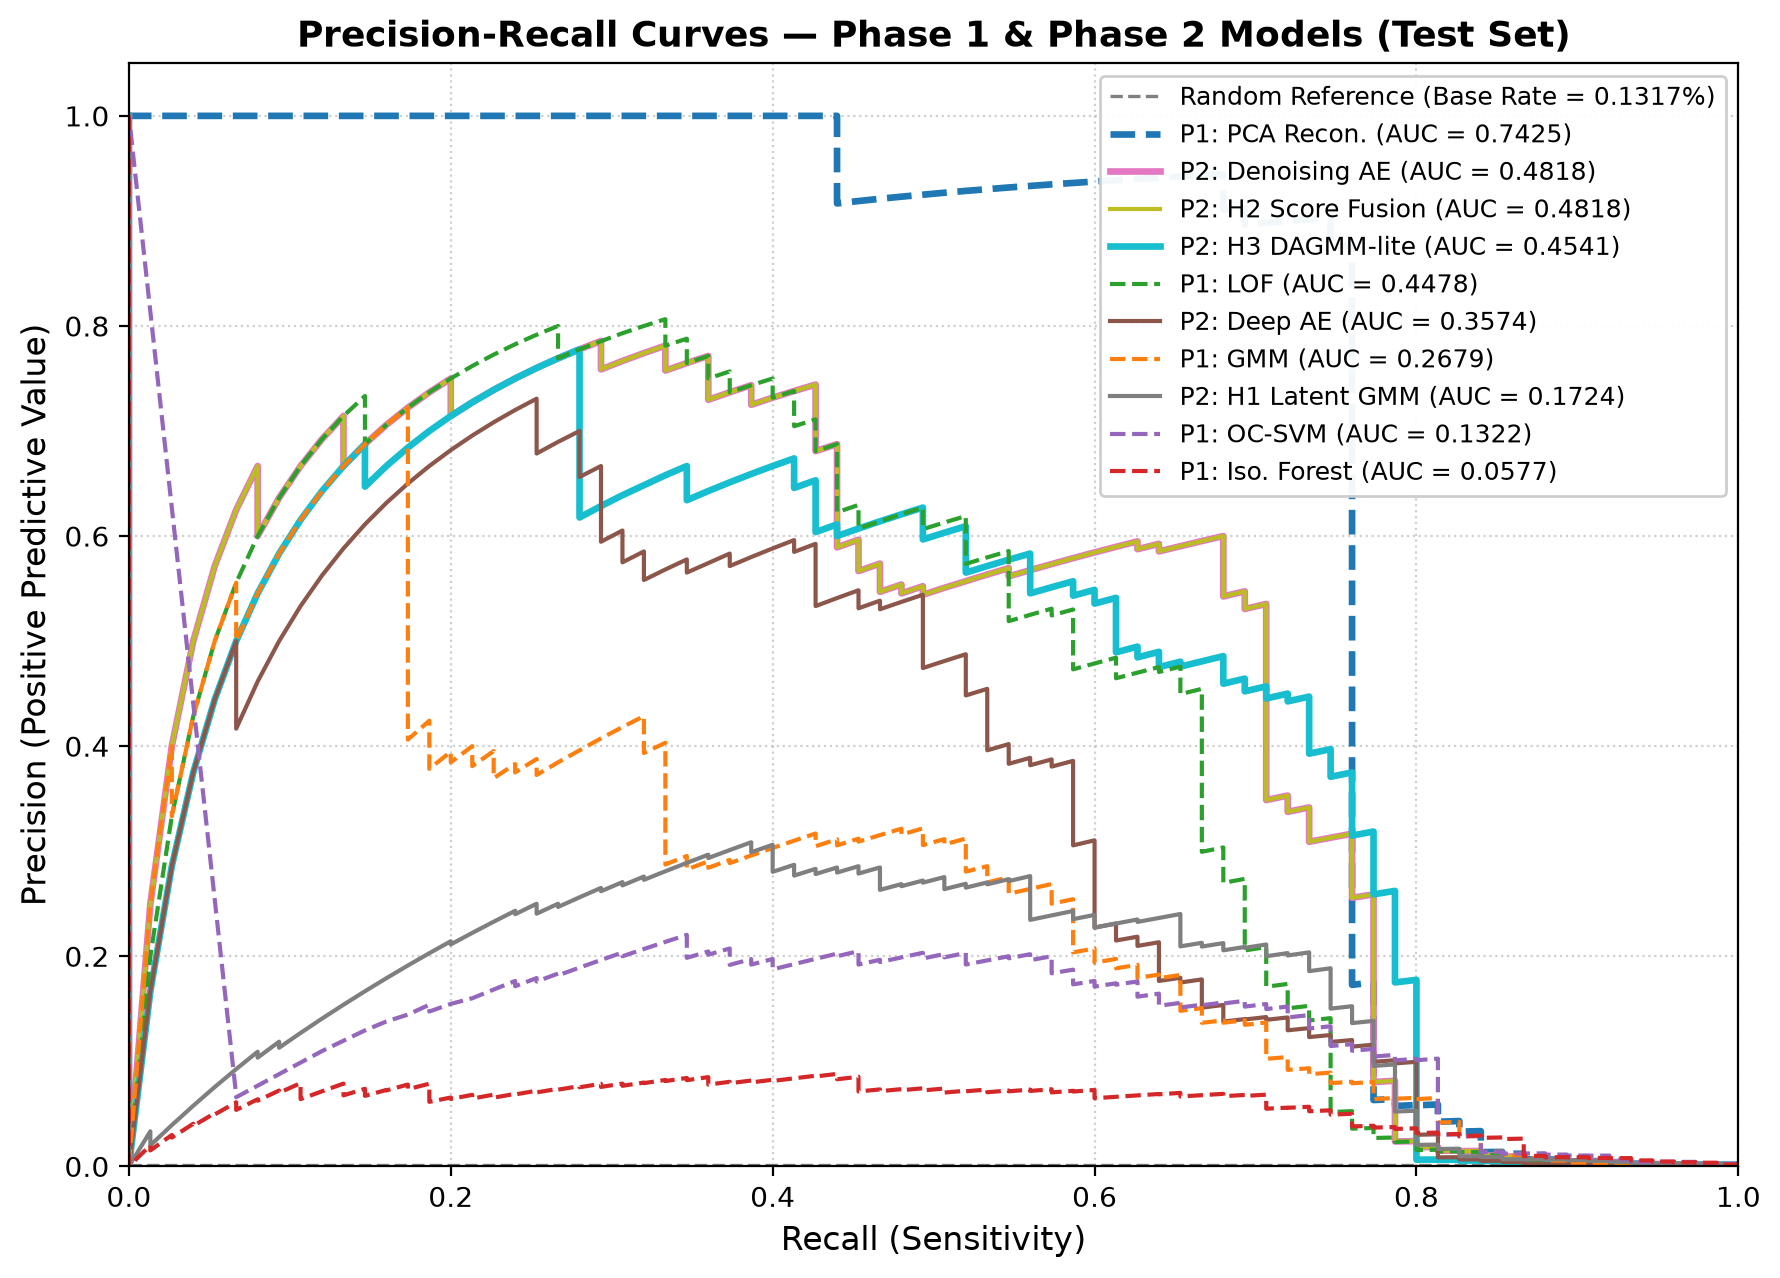
\includegraphics[width=\columnwidth]{final_phase2_pr_curves.png}
\caption{Precision-Recall curves comparing all Phase 1 and Phase 2 models on the untouched chronological test set. The dashed gray line indicates the random baseline ($\text{base rate} = 0.1317\%$).}
\label{fig:final_pr_curves}
\end{figure}

\begin{figure}[t]
\centering
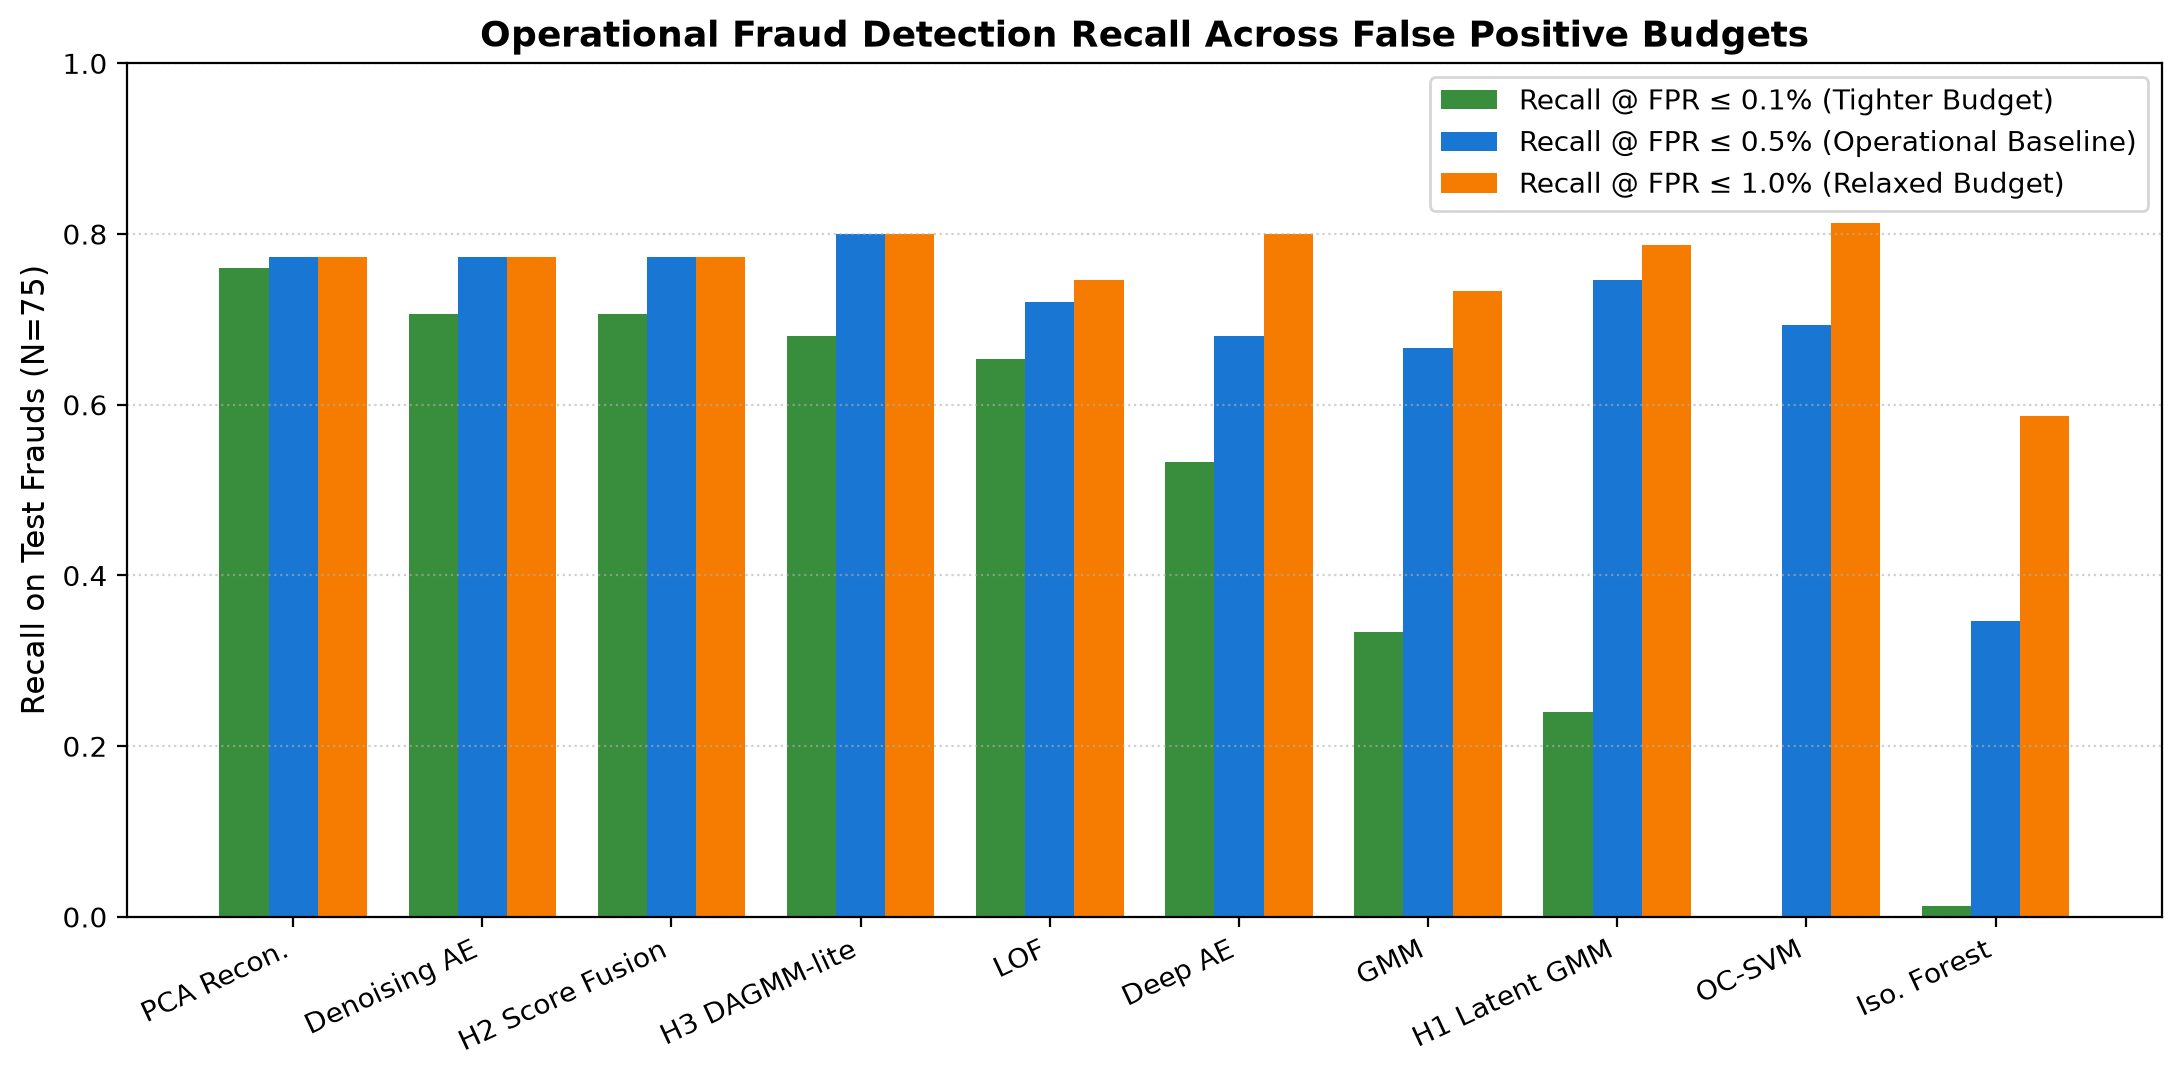
\includegraphics[width=\columnwidth]{final_phase2_recall_at_fpr.png}
\caption{Operational fraud detection recall on test frauds ($N=75$) across operational false positive rate budgets (FPR $\le 0.1\%$, FPR $\le 0.5\%$, FPR $\le 1.0\%$).}
\label{fig:final_recall_bars}
\end{figure}

Fig.~\ref{fig:final_pr_curves} illustrates the precision-recall curves for all models. DAE and DAGMM-lite maintain substantial precision across high-recall operating regimes, comfortably separating themselves from classical density estimation (GMM) and tree partitioning (Isolation Forest). Fig.~\ref{fig:final_recall_bars} breaks down operational recall across fixed FPR budgets.

%%% ─── 12. Discussion & Insights ─────────────────────────────────────────────
\section{Discussion, Theoretical Insights, and Failure Modes}
\label{sec:discussion}

\subsection{Why Does Denoising Autoencoder Outperform Classical GMM?}
DAE ($\text{PR-AUC} = \PRAUCTestDAE{}$) achieves a statistically significant $+0.2139$ PR-AUC improvement over full-space GMM ($p < 0.05$), doubling recall at FPR $\le 0.1\%$ ($70.67\%$ vs.\ $33.33\%$). This advantage stems from the inductive bias established by Vincent \cite{vincent2011connection}: corrupted inputs force the network to estimate the score vector $\nabla_{\mathbf{x}} \log p(\mathbf{x})$, contracting transaction representations onto the nominal manifold. Full-space GMM in $\mathbb{R}^{30}$ suffers from high parameter variance ($465$ parameters per component), causing covariance matrices to become ill-conditioned and diluting density estimation in sparse fraud-prone regions.

\subsection{Why Does Linear PCA Retain the Highest PR-AUC?}
Despite the expressiveness of deep autoencoders, linear PCA reconstruction error remains the top-performing detector ($\text{PR-AUC} = \PRAUCTestPCA{}$). Two primary factors explain this result:
\begin{enumerate}
    \item \textbf{PCA Pre-Anonymized Representation:} The benchmark features $V_1$--$V_{28}$ are already orthogonal principal components generated from an original bank dataset. Legitimate spending behavior is concentrated along linear coordinates.
    \item \textbf{Over-Generalization Pathology:} As Gong et al.\ \cite{gong2019memorizing} established, unconstrained deep neural networks possess universal function approximation capacity. The non-linear decoder partially memorizes and reconstructs anomalous transaction features. Linear PCA has zero capacity to bend non-linearly, penalizing fraud deviations with strictly quadratic residual growth.
\end{enumerate}

\subsection{Why Does Latent GMM (H1) Degrade Detection?}
The failure of standalone latent-space density estimation ($\text{PR-AUC} = \PRAUCTestHOne{}$) illuminates a critical theoretical caveat:
\begin{enumerate}
    \item \textbf{Non-Volume-Preserving Encoder Mapping:} Because the encoder $f_{\boldsymbol{\theta}}: \mathbb{R}^{30} \to \mathbb{R}^8$ has rectangular, non-invertible dimensions, $-\log p(\mathbf{z})$ evaluates density on the *latent coordinate manifold*, not the true data density $p(\mathbf{x})$. Without the Jacobian determinant correction, anomalous transactions are frequently mapped into high-density latent clusters near $\mathbf{z} \approx \mathbf{0}$.
    \item \textbf{Off-Manifold Nature of Credit Card Fraud:} Fraudulent transactions deviate primarily in orthogonal residual directions (high reconstruction error $\|\mathbf{x} - \hat{\mathbf{x}}\|^2$), not in nominal latent coordinates.
\end{enumerate}

\subsection{The Success of DAGMM-lite (H3)}
By combining latent representation $\mathbf{z}$ with reconstruction distance and cosine similarity into an augmented vector $\mathbf{v} = [\mathbf{z}, e^{\text{mse}}, e^{\text{cos}}] \in \mathbb{R}^{10}$, DAGMM-lite resolves H1's blind spot. It achieves **80.00\% recall at FPR $\le 0.5\%$**, outperforming all other models by capturing both directional angle distortion and residual magnitude.

%%% ─── 13. Threats to Validity ───────────────────────────────────────────────
\section{Threats to Validity and Practical Limitations}
\label{sec:threats_validity}

\begin{itemize}
    \item \textbf{Limited Test Fraud Sample ($N=75$):} Although the test partition encompasses 56,962 transactions, the extreme rarity of fraud means only 75 positive events exist, resulting in moderately wide bootstrap confidence intervals ($\pm 0.10$ PR-AUC).
    \item \textbf{PCA-Anonymized Feature Space:} The absence of uncompressed raw transaction attributes (e.g., merchant ID, cardholder historical velocity) limits domain-specific feature engineering.
    \item \textbf{48-Hour Sampling Window:} The dataset represents a two-day snapshot, precluding analysis of multi-day seasonality, pay-cycle surges, or long-term concept drift \cite{lucas2020dataset}.
    \item \textbf{Research Disclaimer:} This system represents an academic benchmark of representation learning under class imbalance and is not certified for standalone production authorization without human analyst oversight.
\end{itemize}

%%% ─── 14. Conclusion & Future Work ──────────────────────────────────────────
\section{Conclusion and Future Work}
\label{sec:conclusion}

In Phase 2 of Project T033, we investigated deep learning and hybrid architectures for unsupervised credit card fraud triage. Our findings demonstrate that Denoising Autoencoders significantly outperform classical Gaussian Mixture Models ($\text{PR-AUC} = \PRAUCTestDAE{}$ vs.\ \PRAUCTestGMM{}, $p < 0.05$) and double fraud catch rates under strict false-alarm budgets. While linear PCA remains the highest standalone detector due to the pre-linear nature of the dataset and autoencoder over-generalization, the decoupled DAGMM-lite hybrid achieves the highest operational recall across all models (\RecallFPRHalfPctHThree{} at $\text{FPR} \le 0.5\%$). Future work will investigate memory-augmented autoencoders (MemAE) to restrict anomalous reconstruction and graph neural network representations to model cardholder-merchant bipartite networks over multi-month transaction streams.

%%% ─── 15. Individual Contributions ──────────────────────────────────────────
\section{Individual Contributions}
\label{sec:contributions}

In accordance with academic integrity guidelines, all team members completed distinct, modular, verified engineering contributions:
\begin{itemize}
    \item \textbf{Kushal Sarkar} (Lead): Pipeline integration, invariant enforcement, score contract testing, master 10-model comparison (`src/final_phase2.py`), final notebook execution (`06b`), slide assembly, and IEEE report coordination.
    \item \textbf{Krishna Pramod Dubale}: Deep learning literature review, theoretical gap analysis, DL data pipeline invariant auditing, and coordinate variance dominance verification (`src/eda_dl.py`).
    \item \textbf{Apoorva Choudhary}: Latent-space GMM formulation, theoretical proofs on change-of-variables and parameter complexity, H1 latent-space grid search, and failure diagnostic analysis (`src/hybrid_latent_gmm.py`).
    \item \textbf{Vani Rudra}: Deep Undercomplete and Denoising Autoencoder architecture design, legitimate-only training pipeline, 5-seed stability validation, and inference latency profiling (`src/autoencoder.py`, `src/train_ae.py`).
    \item \textbf{Prachee Dhar}: Normalized hybrid score fusion (H2), decoupled DAGMM-lite (H3), multi-model overlap Venn analysis, and comprehensive master ablation study (`src/hybrid_fusion.py`, `src/hybrid_dagmm_lite.py`, `src/ablation.py`).
\end{itemize}

%%% ─── References ─────────────────────────────────────────────────────────────
\bibliographystyle{IEEEtran}
\bibliography{refs_phase2}

\end{document}
